\chapter{信赖域}
\label{chap:trust-region}

站在一个点上，手里有目标的梯度和曲率，可以写出一个二次模型，模型的最小点似乎就是下一步该去的地方。可是模型只是在当前点附近展开得到的，走远了它就可能完全失真；曲率不正定时，模型甚至没有最小点。第~\ref{chap:smooth-foundations}章的线搜索先定方向、再定步长，方向一旦定错，步长再怎么调也救不回来。

本章换一个顺序：先问“模型能信多远”，在这个范围内求模型的最小点，方向和长度一起决定，再用真实目标检验模型预测得准不准，据此调整下一轮的范围。这样得到的方法叫\term{信赖域}（trust region）方法。

全章用同一个二维目标把这件事算到底。先写出子问题，看清它的解长什么样；再比较三种便宜的近似求解办法；然后组织完整的迭代，看一步被拒绝时发生什么；最后讨论这套做法能保证什么、不能保证什么，以及它的计算代价。

\section{信赖域模型}
\label{sec:tr-model}

既然局部模型只在一定范围内可靠，怎样把“只在这个范围内相信它”写成一个可以计算的问题？

\paragraph{贯穿全章的例子}
我们用下面这个二维目标：
\begin{equation}
 f(\bm{x})=\frac14x_1^4-\frac12x_1^2+x_1+\frac32x_2^2+x_2.
 \label{eq:tr-example}
\end{equation}
它的梯度和Hessian可以直接写出：
\begin{equation}
 \nabla f(\bm{x})=\begin{bmatrix}x_1^3-x_1+1\\3x_2+1\end{bmatrix},\qquad
 \nabla^2 f(\bm{x})=\begin{bmatrix}3x_1^2-1&0\\0&3\end{bmatrix}.
 \label{eq:tr-example-derivatives}
\end{equation}

令梯度为零，第二个分量给出$x_2=-1/3$，第一个分量是三次方程$x_1^3-x_1+1=0$，它只有一个实根$x_1\approx-1.3247$。这个驻点处Hessian正定，$f$又随$\lVert\bm{x}\rVert_2\to\infty$趋于正无穷，所以它就是全局最小点：
\[
 \bm{x}^\star\approx(-1.3247,\,-0.3333)^\top,\qquad f^\star\approx-1.5989.
\]

全章反复用到两个点。一个是$\bm{a}=(2,2)^\top$，这里Hessian正定，数据是
\begin{equation}
 f(\bm{a})=12,\qquad \bm{g}=\begin{bmatrix}7\\7\end{bmatrix},\qquad \bm{B}=\begin{bmatrix}11&0\\0&3\end{bmatrix}.
 \label{eq:tr-data-a}
\end{equation}
另一个是原点，这里Hessian不定，数据是
\begin{equation}
 f(\bm{0})=0,\qquad \bm{g}=\begin{bmatrix}1\\1\end{bmatrix},\qquad \bm{B}=\begin{bmatrix}-1&0\\0&3\end{bmatrix}.
 \label{eq:tr-data-o}
\end{equation}

\paragraph{模型能信多远}
在当前点$\bm{x}^{(t)}$展开到二阶，用位移$\bm{p}$作自变量，就得到\term{二次模型}（quadratic model）：
\begin{equation}
 m^{(t)}(\bm{p})=f(\bm{x}^{(t)})+\langle\bm{g}^{(t)},\bm{p}\rangle+\frac12\bm{p}^\top\bm{B}^{(t)}\bm{p}.
 \label{eq:tr-model}
\end{equation}
其中$\bm{g}^{(t)}=\nabla f(\bm{x}^{(t)})$，$\bm{B}^{(t)}$是对称矩阵，可以取Hessian $\bm{H}^{(t)}$，也可以取第~\ref{chap:quasi-newton}章由梯度差构造的近似。本节取$\bm{B}^{(t)}=\bm{H}^{(t)}$。

模型与目标差多少？例中$x_2$部分本来就是二次的，没有误差；$x_1$部分由四次多项式的展开直接得到，当$\bm{B}$取Hessian时
\begin{equation}
 f(\bm{x}+\bm{p})-m(\bm{p})=x_1p_1^3+\frac14p_1^4.
 \label{eq:tr-example-error}
\end{equation}

误差随$\lvert p_1\rvert$的增大而迅速增大。$\lvert p_1\rvert$很小时，高阶项微不足道；$\lvert p_1\rvert$到了$2$，在原点误差就是$4$，已经超过这里函数值变化的量级。图~\ref{fig:tr-model-slice}沿$x_1$方向画出了这件事，浅蓝带表示模型大致可信的范围。

\begin{BookInlineFigure}
 \centering
 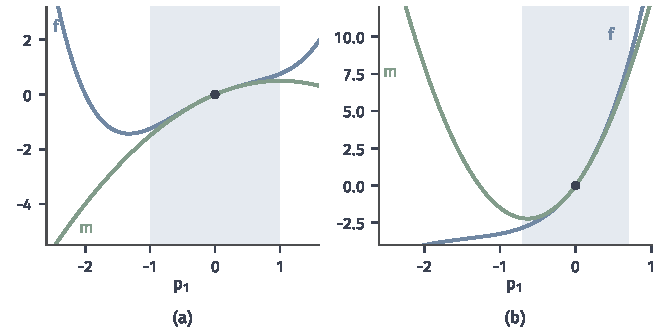
\includegraphics[width=112mm]{figures/05-optimization/02-smooth-optimization/matplotlib/tr-model-slice/figure.pdf}
 \caption{目标~\eqref{eq:tr-example}的$x_1$部分（蓝）与二次模型（绿）沿$p_1$的比较，黑点是展开点，浅蓝带是两者大致重合的范围。(a)~在$x_1=0$展开，曲率为负，模型向左无限下降，而目标很快转头向上。(b)~在$x_1=2$展开，曲率为正，模型有最小点，但左侧的目标比模型低得多。}
 \label{fig:tr-model-slice}
\end{BookInlineFigure}

图~\ref{fig:tr-model-contours}在平面上比较同一件事。在点$\bm{a}$附近，两组等高线几乎一样；离开圆盘之后，目标的等高线向左拉伸，模型仍是一组椭圆。

\begin{BookInlineFigure}
 \centering
 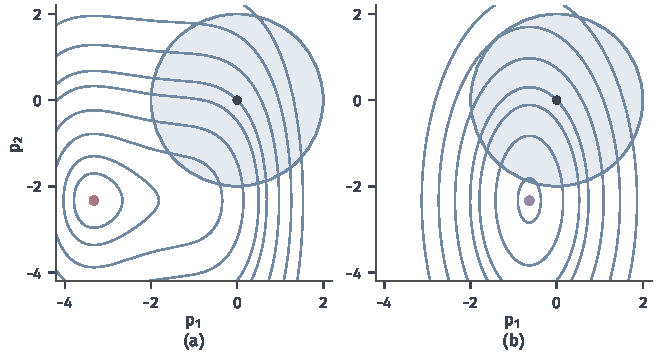
\includegraphics[width=112mm]{figures/05-optimization/02-smooth-optimization/matplotlib/tr-model-contours/figure.pdf}
 \caption{以$\bm{a}=(2,2)^\top$为原点的位移坐标下的等高线（蓝）。(a)~真实目标，红点是最小点。(b)~二次模型，紫点是模型的最小点。浅蓝圆盘半径为$2$，圆盘内两图相近，圆盘外差别明显。}
 \label{fig:tr-model-contours}
\end{BookInlineFigure}

\paragraph{子问题}
既然模型只在附近可靠，就只在附近找它的最小点。给定半径$\Delta^{(t)}>0$，定义\term{信赖域子问题}（trust-region subproblem）：
\begin{equation}
 \min_{\bm{p}\in\mathbb{R}^n}\ m^{(t)}(\bm{p})\qquad\text{满足}\quad\lVert\bm{p}\rVert_2\leq\Delta^{(t)}.
 \label{eq:tr-subproblem}
\end{equation}
半径$\Delta^{(t)}$约束的是这一轮的位移，原问题仍然是无约束的。下一轮换一个点、换一个半径，约束也跟着换。

半径的含义可以用一张手绘地图来理解。地图是在当前位置附近勘测的（对应二次模型），周围画得准，远处多半是推测。你决定只按地图走到某个距离为止（对应半径），走到后核对实地与地图是否相符，相符就下次敢走远些，不符就走近些（对应后面的半径更新）。这个类比有一处不贴切：半径并不是模型真实误差的边界，它只是算法根据最近的核对结果作出的估计，可能偏大，也可能偏小。

\paragraph{曲率不正定时}
第~\ref{chap:second-order-methods}章的Newton法要解$\bm{B}\bm{d}=-\bm{g}$。原点的数据~\eqref{eq:tr-data-o}上这个方程仍可解，解是
\[
 \bm{d}^{\mathrm{N}}=-\bm{B}^{-1}\bm{g}=\begin{bmatrix}1\\-1/3\end{bmatrix}.
\]

它与梯度的内积决定这个方向是上坡还是下坡：
\[
 \langle\bm{g},\bm{d}^{\mathrm{N}}\rangle=1-\frac13=\frac23>0.
\]
内积为正，这个方向是上坡方向。$\bm{d}^{\mathrm{N}}$只是模型的驻点，模型在这里是个鞍面。沿$\bm{d}^{\mathrm{N}}$作线搜索不会有任何下降的步长，所以线搜索框架不得不先修改$\bm{B}$，使它正定。

信赖域子问题没有这个麻烦。闭球是紧集，$m$连续，所以无论$\bm{B}$是否正定，最小点都存在。例中模型沿$p_1$轴是$p_1-p_1^2/2$，向左无限下降，无约束时没有最小点；加上半径之后，解就落在球的边界上。图~\ref{fig:tr-newton-ascent}画出了$\Delta=2$的情形：$\bm{B}$无需修改，负曲率反而被利用，它把解推向了边界。

\begin{BookInlineFigure}
 \centering
 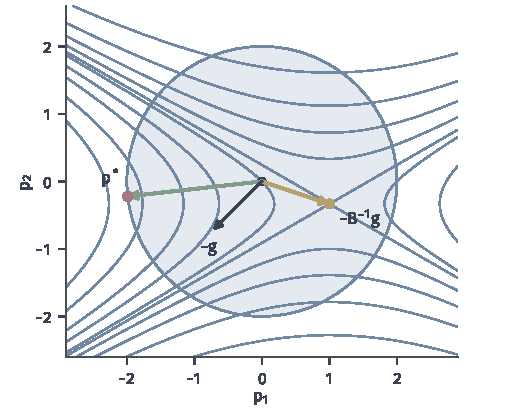
\includegraphics[width=88mm]{figures/05-optimization/02-smooth-optimization/matplotlib/tr-newton-ascent/figure.pdf}
 \caption{原点处的二次模型，蓝线是等高线，浅蓝圆盘半径$\Delta=2$。黄色箭头指向模型的驻点$-\bm{B}^{-1}\bm{g}$，黑色箭头是负梯度方向，红点是子问题的全局解$\bm{p}^\star$，绿色箭头指向它。黄色方向是上坡方向，而子问题的解利用负曲率走到了圆盘左侧边界。}
 \label{fig:tr-newton-ascent}
\end{BookInlineFigure}

\paragraph{与线搜索的对照}
第~\ref{chap:smooth-foundations}章的线搜索分两步：先选定下降方向$\bm{d}^{(t)}$，再沿这条射线选步长$\alpha^{(t)}$。信赖域把顺序倒过来：先选定半径，再同时决定方向和长度。半径变了，步的方向也跟着变。

在点$\bm{a}$，图~\ref{fig:tr-line-vs-region}画出了两者的差别。线搜索的候选点都在一条射线上；信赖域的解随半径变化走出一条曲线，半径小时贴近负梯度方向，半径大时转向Newton点。半径的调整因此比步长的调整多一层作用，它还在改变方向。

\begin{BookInlineFigure}
 \centering
 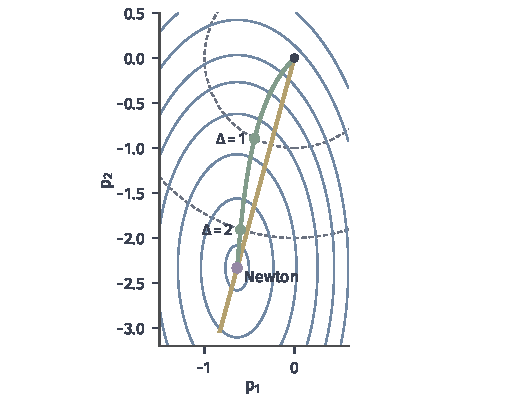
\includegraphics[width=86mm]{figures/05-optimization/02-smooth-optimization/matplotlib/tr-line-vs-region/figure.pdf}
 \caption{点$\bm{a}$处的二次模型等高线（蓝）。黄线是沿Newton方向的射线，线搜索只在这条线上选点。绿线是子问题的全局解随$\Delta$变化的轨迹，绿点是$\Delta=1$和$\Delta=2$时的解，虚线圆是对应的边界，紫点是Newton点。}
 \label{fig:tr-line-vs-region}
\end{BookInlineFigure}

表~\ref{tab:tr-vs-linesearch}把两种做法并列。

\begin{BookInlineTable}
 \centering
 \begin{tabular}{lll}
  \toprule
  & 线搜索 & 信赖域\\
  \midrule
  先固定的量 & 方向$\bm{d}^{(t)}$ & 半径$\Delta^{(t)}$\\
  后决定的量 & 步长$\alpha^{(t)}$ & 位移$\bm{p}^{(t)}$（方向和长度）\\
  $\bm{B}$的要求 & 需要给出下降方向 & 对称即可\\
  一次试探失败 & 缩短步长，方向不变 & 缩小半径，方向可变\\
  \bottomrule
 \end{tabular}
 \caption{线搜索与信赖域的分工对照。}
 \label{tab:tr-vs-linesearch}
\end{BookInlineTable}

\paragraph{子问题的全局解}
子问题虽然非凸，它的全局解却有干净的刻画。下面的定理说明，解满足一个被平移过的线性方程，平移量$\lambda$恰好使矩阵半正定。

\begin{theorem}[子问题的全局解]
 \label{thm:tr-exact}
 设$\bm{B}$对称，$\Delta>0$，$m$如式~\eqref{eq:tr-model}（省略上标$(t)$）。点$\bm{p}^\star$是子问题~\eqref{eq:tr-subproblem}的全局解，当且仅当$\lVert\bm{p}^\star\rVert_2\leq\Delta$，并且存在$\lambda\geq0$，使得
 \begin{equation}
  (\bm{B}+\lambda\bm{I})\bm{p}^\star=-\bm{g},\qquad
  \lambda(\Delta-\lVert\bm{p}^\star\rVert_2)=0,\qquad
  \bm{B}+\lambda\bm{I}\succeq\bm{0}.
  \label{eq:tr-exact-conditions}
 \end{equation}
\end{theorem}

\begin{proof}
 先证充分性。令
 \[
  \hat{m}(\bm{p})=m(\bm{p})+\frac{\lambda}{2}\lVert\bm{p}\rVert_2^2.
 \]
 它的Hessian是$\bm{B}+\lambda\bm{I}\succeq\bm{0}$，所以是凸函数；式~\eqref{eq:tr-exact-conditions}的第一式说明$\nabla\hat{m}(\bm{p}^\star)=\bm{0}$，因此$\bm{p}^\star$是$\hat{m}$的全局最小点。对任意$\lVert\bm{p}\rVert_2\leq\Delta$，把$\hat{m}(\bm{p})\geq\hat{m}(\bm{p}^\star)$展开，得到
 \[
  m(\bm{p})\geq m(\bm{p}^\star)+\frac{\lambda}{2}\bigl(\lVert\bm{p}^\star\rVert_2^2-\lVert\bm{p}\rVert_2^2\bigr).
 \]
 若$\lambda=0$，右端就是$m(\bm{p}^\star)$。若$\lambda>0$，第二式给出$\lVert\bm{p}^\star\rVert_2=\Delta$，括号非负。两种情形都有$m(\bm{p})\geq m(\bm{p}^\star)$。

 再证必要性。若$\lVert\bm{p}^\star\rVert_2<\Delta$，$\bm{p}^\star$是二次函数的内部局部极小点，于是梯度$\bm{B}\bm{p}^\star+\bm{g}=\bm{0}$，Hessian $\bm{B}\succeq\bm{0}$，取$\lambda=0$即可。

 下设$\lVert\bm{p}^\star\rVert_2=\Delta$，分三步。第一步找乘子。任取与$\bm{p}^\star$正交的单位向量$\bm{v}$，下面的曲线落在球面上：
 \[
  \bm{q}(\theta)=\cos\theta\,\bm{p}^\star+\Delta\sin\theta\,\bm{v}.
 \]
 $\theta=0$时函数$m(\bm{q}(\theta))$最小，导数为零：
 \[
  \Delta\,\langle\bm{B}\bm{p}^\star+\bm{g},\bm{v}\rangle=0.
 \]
 所以$\bm{B}\bm{p}^\star+\bm{g}$与所有切向量正交，它只能是$\bm{p}^\star$的倍数，记为$-\lambda\bm{p}^\star$，这就是第一式。

 第二步证$\lambda\geq0$。对$s\in[0,1]$，点$(1-s)\bm{p}^\star$可行，$m((1-s)\bm{p}^\star)$在$s=0$的右导数不能为负：
 \[
  -\langle\bm{B}\bm{p}^\star+\bm{g},\bm{p}^\star\rangle=\lambda\Delta^2\geq0.
 \]

 第三步证半正定。$\hat{m}$是二次函数且在$\bm{p}^\star$处梯度为零，所以
 \[
  \hat{m}(\bm{p})-\hat{m}(\bm{p}^\star)=\frac12(\bm{p}-\bm{p}^\star)^\top(\bm{B}+\lambda\bm{I})(\bm{p}-\bm{p}^\star).
 \]
 当$\lVert\bm{p}\rVert_2=\Delta$时，$\hat{m}$与$m$的差相同，而$m(\bm{p})\geq m(\bm{p}^\star)$，于是
 \[
  (\bm{p}-\bm{p}^\star)^\top(\bm{B}+\lambda\bm{I})(\bm{p}-\bm{p}^\star)\geq0.
 \]
 任取满足$\langle\bm{w},\bm{p}^\star\rangle\neq0$的$\bm{w}$，令
 \[
  \bm{p}=\bm{p}^\star-2\frac{\langle\bm{w},\bm{p}^\star\rangle}{\langle\bm{w},\bm{w}\rangle}\bm{w}.
 \]
 这是$\bm{p}^\star$关于$\bm{w}$的法平面的反射，长度仍为$\Delta$，而$\bm{p}-\bm{p}^\star$与$\bm{w}$平行，所以$\bm{w}^\top(\bm{B}+\lambda\bm{I})\bm{w}\geq0$。满足$\langle\bm{w},\bm{p}^\star\rangle\neq0$的$\bm{w}$在$\mathbb{R}^n$中稠密，由连续性，不等式对所有$\bm{w}$成立。
\end{proof}

三个条件各有作用。第一式说明解是一个被“加了$\lambda$”的Newton方程的解，$\lambda$越大，方程越接近$\lambda\bm{p}=-\bm{g}$，解越贴近负梯度方向。第二式说明半径不起作用时$\lambda=0$，解就是Newton点。第三式是全局性的来源：它要求$\lambda$至少抵消最负的特征值，只满足前两式的点可能只是局部解或驻点。

$\lambda$的作用类似预算约束下的影子价格：半径限得越紧，$\lambda$越大。这个类比只说明单调关系，$\lambda$的单位与目标值的单位并不相同。

\paragraph{怎样求$\lambda$}
设$\bm{B}$的特征值为$\lambda_1\leq\cdots\leq\lambda_n$，对应的单位正交特征向量为$\bm{q}_1,\ldots,\bm{q}_n$。当$\lambda>\max\{0,-\lambda_1\}$时，式~\eqref{eq:tr-exact-conditions}的第一式有唯一解$\bm{p}(\lambda)$，它的长度满足
\begin{equation}
 \lVert\bm{p}(\lambda)\rVert_2^2=\sum_{i=1}^n\frac{\langle\bm{q}_i,\bm{g}\rangle^2}{(\lambda_i+\lambda)^2}.
 \label{eq:tr-secular}
\end{equation}
每一项都随$\lambda$严格减小（只要系数不为零）。求解子问题于是化为一元方程$\lVert\bm{p}(\lambda)\rVert_2=\Delta$，称为\term{久期方程}（secular equation）。

点$\bm{a}$的数据~\eqref{eq:tr-data-a}上，取$\Delta=2$，式~\eqref{eq:tr-secular}成为
\[
 \lVert\bm{p}(\lambda)\rVert_2^2=\frac{49}{(11+\lambda)^2}+\frac{49}{(3+\lambda)^2}.
\]

$\lambda=0$时长度约为$2.419$，大于$\Delta$，Newton点在球外，所以$\lambda>0$。再试几个值：
\[
 \lVert\bm{p}(0.5)\rVert_2\approx2.091,\qquad
 \lVert\bm{p}(0.7)\rVert_2\approx1.984,\qquad
 \lVert\bm{p}(0.67)\rVert_2\approx1.9995.
\]

继续缩小区间，得到$\lambda\approx0.669$，相应的解是
\[
 \bm{p}^\star\approx(-0.600,\,-1.908)^\top.
\]
实际计算不用谱分解，而是对几个试探的$\lambda$作Cholesky分解，用Newton迭代解$1/\lVert\bm{p}(\lambda)\rVert_2=1/\Delta$；这个函数比长度本身更接近线性，几次迭代就够了。

图~\ref{fig:tr-secular}(a)是这条曲线。原点的数据上（图~\ref{fig:tr-secular}(b)），$\bm{B}$有负特征值$-1$，只能在$\lambda>1$的范围内找解。曲线在$\lambda=1$处趋于无穷，所以对任何半径都有交点，$\Delta=2$时$\lambda\approx1.503$。

\begin{BookInlineFigure}
 \centering
 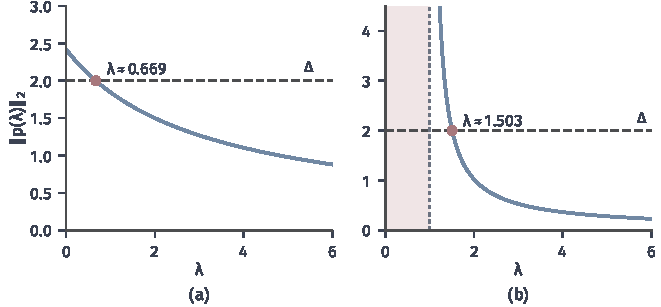
\includegraphics[width=112mm]{figures/05-optimization/02-smooth-optimization/matplotlib/tr-secular/figure.pdf}
 \caption{解的长度$\lVert\bm{p}(\lambda)\rVert_2$（蓝）与半径$\Delta=2$（虚线）的交点（红）给出乘子。(a)~点$\bm{a}$，$\bm{B}$正定，曲线从Newton步的长度开始下降。(b)~原点，$\bm{B}$的最小特征值为$-1$，红色浅底的区域$\lambda<1$不满足$\bm{B}+\lambda\bm{I}\succeq\bm{0}$。}
 \label{fig:tr-secular}
\end{BookInlineFigure}

\paragraph{困难情形}
上面的论证依赖$\langle\bm{q}_1,\bm{g}\rangle\neq0$。如果梯度与最小特征值的特征空间正交，式~\eqref{eq:tr-secular}中对应的项消失，曲线在$\lambda=-\lambda_1$处不再趋于无穷，久期方程可能无解。这称为子问题的\term{困难情形}（hard case）。

看下面这组数据：
\[
 \bm{g}=\begin{bmatrix}0\\1\end{bmatrix},\qquad\bm{B}=\begin{bmatrix}-1&0\\0&3\end{bmatrix},\qquad\Delta=1.
\]

当$\lambda>1$时，第一式给出的解是
\[
 \bm{p}(\lambda)=\begin{bmatrix}0\\-1/(\lambda+3)\end{bmatrix},
\]
长度小于$1/4$，够不到边界。定理~\ref{thm:tr-exact}要求$\lambda\geq1$，所以只能取$\lambda=1$。此时$\bm{B}+\bm{I}=\operatorname{diag}(0,4)$奇异，方程的解不唯一：
\[
 \bm{p}=\begin{bmatrix}\tau\\-1/4\end{bmatrix},\qquad\tau\in\mathbb{R}.
\]

沿奇异方向补足长度，使$\lVert\bm{p}\rVert_2=1$，得到两个全局解：
\[
 \tau=\pm\frac{\sqrt{15}}{4},\qquad m(\bm{p})-m(\bm{0})=-\frac58.
\]
图~\ref{fig:tr-hard-case}比较了$g_1$很小与$g_1=0$两种情形。$g_1=0.1$时交点贴近$\lambda=1$；$g_1$恰好为零时，曲线在$\lambda=1$处停在$1/4$，交点消失，解要靠特征向量补足。

\begin{BookInlineFigure}
 \centering
 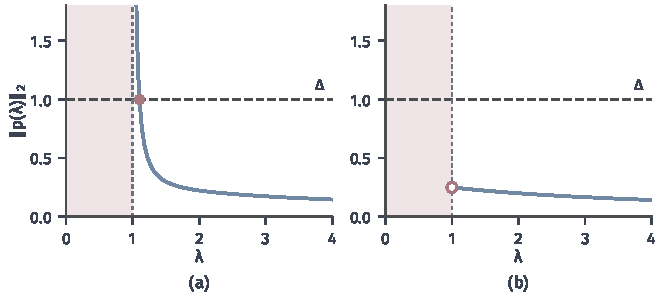
\includegraphics[width=112mm]{figures/05-optimization/02-smooth-optimization/matplotlib/tr-hard-case/figure.pdf}
 \caption{$\bm{B}=\operatorname{diag}(-1,3)$，$\Delta=1$（虚线）时的解长度（蓝）。(a)~$\bm{g}=(0.1,1)^\top$，曲线在$\lambda=1$处趋于无穷，有交点。(b)~$\bm{g}=(0,1)^\top$，曲线只到$1/4$（空心点），与虚线不相交，这是困难情形。}
 \label{fig:tr-hard-case}
\end{BookInlineFigure}

\paragraph{三个不同的量}
子问题的解、模型的下降、真实目标的下降是三件事，下面把它们分开。对候选步$\bm{p}$，定义\term{预测下降}（predicted reduction）和\term{实际下降}（actual reduction）：
\begin{equation}
 \operatorname{pred}(\bm{p})=m(\bm{0})-m(\bm{p}),\qquad
 \operatorname{ared}(\bm{p})=f(\bm{x})-f(\bm{x}+\bm{p}).
 \label{eq:tr-pred-ared}
\end{equation}

子问题的全局解使预测下降最大，却未必使实际下降最大。在原点取$\Delta=2$，全局解是$\bm{p}^\star\approx(-1.988,-0.222)^\top$。由式~\eqref{eq:tr-example-error}，它的模型误差大约是$\tfrac14(1.988)^4\approx3.90$，于是
\[
 \operatorname{pred}(\bm{p}^\star)\approx4.111,\qquad
 \operatorname{ared}(\bm{p}^\star)\approx0.209.
\]

再看同一个球内的另一个点$\bm{p}=(-1.6,-1.2)^\top$。它的预测下降小得多，实际下降反而大一些：
\[
 \operatorname{pred}(\bm{p})=1.92,\qquad
 \operatorname{ared}(\bm{p})\approx0.282.
\]

这个对比说明，模型下降的大小只是在模型的范围内才有意义。图~\ref{fig:tr-three-decreases}画出全局解的两种下降随半径的变化：半径小时两条曲线重合，半径大时预测下降继续上升，实际下降掉头向下。预测和实际的差距正是调整半径的依据，后面第~\ref{sec:tr-acceptance}节用它们的比值组织迭代。

\begin{BookInlineFigure}
 \centering
 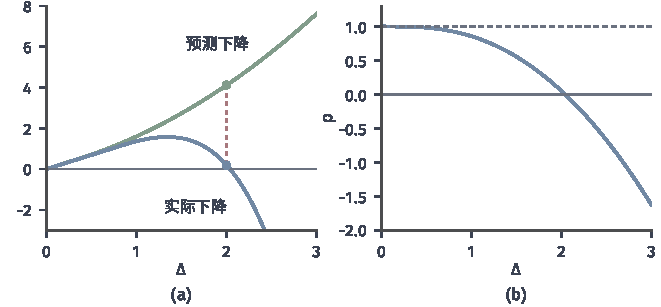
\includegraphics[width=112mm]{figures/05-optimization/02-smooth-optimization/matplotlib/tr-three-decreases/figure.pdf}
 \caption{原点处子问题全局解随半径的变化。(a)~预测下降（绿）与实际下降（蓝），红色虚线标出$\Delta=2$处的差距。(b)~实际下降与预测下降之比$\rho$（蓝），半径越大越偏离$1$，在$\Delta$约为$2$时降到零附近。}
 \label{fig:tr-three-decreases}
\end{BookInlineFigure}

\section{子问题的求解}
\label{sec:tr-subproblem}

第~\ref{sec:tr-model}节的刻画需要分解$\bm{B}+\lambda\bm{I}$好几次，每一轮外层迭代都这样做，代价可能比外层本身还高。接下来要弄清：能否用便宜得多的办法得到一个“够用”的步？

下面对同一个模型和同一个半径比较三种计算。它们是：只沿负梯度取步、把负梯度步与Newton步连起来、用共轭梯度迭代逐步逼近。主例取点$\bm{a}$的数据~\eqref{eq:tr-data-a}，半径$\Delta=2$；Hessian不定的情形用原点的数据~\eqref{eq:tr-data-o}。外层迭代真正需要的，不是子问题的精确解，而是模型下降达到一个规定的比例。这个比例由最简单的那种步来给出。

本节所有量都在同一轮外层迭代内，省略上标$(t)$，写$m,\bm{g},\bm{B},\Delta$。

\subsection{Cauchy步}
\label{sec:tr-cauchy}

\paragraph{沿负梯度最小化模型}
最便宜的做法是只在负梯度这条射线上找模型的最小点。设$\bm{g}\neq\bm{0}$，把点写成$\bm{p}=-a\,\bm{g}/\lVert\bm{g}\rVert_2$，其中$a\in[0,\Delta]$是走过的长度。令
\[
 \kappa=\frac{\bm{g}^\top\bm{B}\bm{g}}{\lVert\bm{g}\rVert_2^2},
\]
它是模型沿负梯度方向的曲率。代入式~\eqref{eq:tr-model}，模型的变化量是一元二次函数
\begin{equation}
 \psi(a)=m\Bigl(-a\frac{\bm{g}}{\lVert\bm{g}\rVert_2}\Bigr)-m(\bm{0})=-a\lVert\bm{g}\rVert_2+\frac{\kappa}{2}a^2.
 \label{eq:tr-cauchy-psi}
\end{equation}

在$[0,\Delta]$上最小化$\psi$，分两种情形。若$\kappa\leq0$，$\psi$严格递减，应当走到边界$a=\Delta$。若$\kappa>0$，$\psi$的顶点在$a=\lVert\bm{g}\rVert_2/\kappa$，它在区间内就取顶点，否则截断在边界。合起来就得到\term{Cauchy步}（Cauchy step）的长度，步本身记为$\bm{p}^{\mathrm{C}}$：
\begin{equation}
 \bm{p}^{\mathrm{C}}=-a^{\mathrm{C}}\frac{\bm{g}}{\lVert\bm{g}\rVert_2},\qquad
 a^{\mathrm{C}}=
 \begin{cases}
  \Delta,&\kappa\leq0,\\
  \min\{\Delta,\ \lVert\bm{g}\rVert_2/\kappa\},&\kappa>0.
 \end{cases}
 \label{eq:tr-cauchy-step}
\end{equation}
图~\ref{fig:tr-cauchy-cases}画出三种情形。计算时只需要一次矩阵向量乘积$\bm{B}\bm{g}$。

\begin{BookInlineFigure}
 \centering
 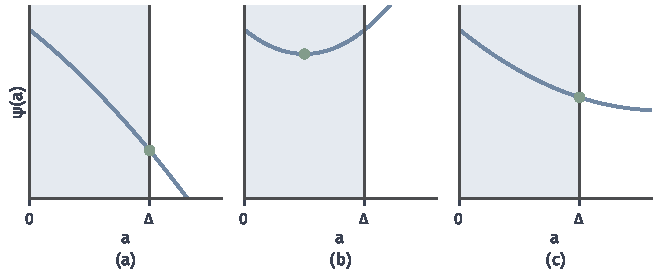
\includegraphics[width=112mm]{figures/05-optimization/02-smooth-optimization/matplotlib/tr-cauchy-cases/figure.pdf}
 \caption{函数$\psi(a)$（蓝）的三种情形，浅蓝带是可取的范围，深灰线是边界，绿点是Cauchy步的长度。(a)~$\kappa\leq0$，走到边界。(b)~$\kappa>0$且顶点在区间内，取顶点。(c)~$\kappa>0$但顶点在区间外，截断在边界。}
 \label{fig:tr-cauchy-cases}
\end{BookInlineFigure}

点$\bm{a}$的数据上，$\bm{g}^\top\bm{B}\bm{g}=49\times14=686$，$\lVert\bm{g}\rVert_2^2=98$，所以
\[
 \kappa=7,\qquad\lVert\bm{g}\rVert_2=7\sqrt2,\qquad\frac{\lVert\bm{g}\rVert_2}{\kappa}=\sqrt2.
\]

半径$\Delta=2$大于$\sqrt2$，Cauchy步取顶点：
\[
 \bm{p}^{\mathrm{C}}=-\sqrt2\cdot\frac{(7,7)^\top}{7\sqrt2}=\begin{bmatrix}-1\\-1\end{bmatrix},\qquad
 \operatorname{pred}(\bm{p}^{\mathrm{C}})=7\sqrt2\cdot\sqrt2-\frac72\cdot2=7.
\]
半径若取$\Delta=1$，则截断在边界，$a^{\mathrm{C}}=1$，预测下降为$7\sqrt2-3.5\approx6.40$。

\paragraph{Cauchy步提供的模型下降}
Cauchy步便宜，它的价值却在于给出了一条有保证的下限。下面的引理说明，它的预测下降由梯度大小、半径和曲率上界控制。

\begin{lemma}[Cauchy步的下降量]
 \label{lem:tr-cauchy-decrease}
 设$\bm{g}\neq\bm{0}$，$\bm{B}$对称。Cauchy步满足
 \begin{equation}
  \operatorname{pred}(\bm{p}^{\mathrm{C}})\geq\frac12\lVert\bm{g}\rVert_2\min\Bigl\{\Delta,\ \frac{\lVert\bm{g}\rVert_2}{\lVert\bm{B}\rVert_2}\Bigr\},
  \label{eq:tr-cauchy-decrease}
 \end{equation}
 其中$\bm{B}=\bm{0}$时第二项理解为$+\infty$。
\end{lemma}

\begin{proof}
 由式~\eqref{eq:tr-cauchy-psi}，预测下降是
 \[
  \operatorname{pred}(\bm{p}^{\mathrm{C}})=a^{\mathrm{C}}\lVert\bm{g}\rVert_2-\frac{\kappa}{2}(a^{\mathrm{C}})^2,
 \]
 并且$\kappa\leq\lVert\bm{B}\rVert_2$。按三种情形估计。

 若$\kappa\leq0$，则$a^{\mathrm{C}}=\Delta$，第二项非负，所以
 \[
  \operatorname{pred}(\bm{p}^{\mathrm{C}})\geq\Delta\lVert\bm{g}\rVert_2.
 \]

 若$\kappa>0$且$\lVert\bm{g}\rVert_2/\kappa\leq\Delta$，则取顶点，所以
 \[
  \operatorname{pred}(\bm{p}^{\mathrm{C}})=\frac{\lVert\bm{g}\rVert_2^2}{2\kappa}\geq\frac{\lVert\bm{g}\rVert_2^2}{2\lVert\bm{B}\rVert_2}.
 \]

 若$\kappa>0$且$\lVert\bm{g}\rVert_2/\kappa>\Delta$，则$a^{\mathrm{C}}=\Delta$，并且$\kappa\Delta<\lVert\bm{g}\rVert_2$，所以
 \[
  \operatorname{pred}(\bm{p}^{\mathrm{C}})=\Delta\lVert\bm{g}\rVert_2-\frac{\kappa\Delta}{2}\Delta\geq\frac12\Delta\lVert\bm{g}\rVert_2.
 \]
 三种情形都不小于式~\eqref{eq:tr-cauchy-decrease}的右端。
\end{proof}

点$\bm{a}$的数据上$\lVert\bm{B}\rVert_2=11$，取$\Delta=2$，式~\eqref{eq:tr-cauchy-decrease}的右端是
\[
 \frac12\cdot7\sqrt2\cdot\min\Bigl\{2,\ \frac{7\sqrt2}{11}\Bigr\}=\frac{49}{11}\approx4.45,
\]
确实不超过实际的预测下降$7$。这个下限比实际值松，它的用处在于对所有模型一致成立。

这条下限只用到一阶信息和曲率的上界，$\bm{B}$可以不定。我们把它提升为对任意候选步的要求：若存在常数$c_1\in(0,1]$，使得
\begin{equation}
 \operatorname{pred}(\bm{p})\geq c_1\lVert\bm{g}\rVert_2\min\Bigl\{\Delta,\ \frac{\lVert\bm{g}\rVert_2}{\lVert\bm{B}\rVert_2}\Bigr\},
 \label{eq:tr-sufficient-decrease}
\end{equation}
就说$\bm{p}$达到\term{充分模型下降}（sufficient model decrease）。第~\ref{sec:tr-convergence}节会看到，一阶收敛只需要这一条；任何预测下降不低于Cauchy步的求解器，都自动满足它，$c_1=1/2$。

要分清这条保障和精确求解的差别。式~\eqref{eq:tr-sufficient-decrease}只是一条下限，并不表示接近子问题的最优值。点$\bm{a}$上Cauchy步的预测下降是$7$，全局解是$10.115$；原点上$\Delta=2$时，Cauchy步是$1$，全局解是$4.111$。只用Cauchy步的方法本质上是最速下降，保留了收敛性，也保留了最速下降的慢。下面两种办法都从它出发，再往前走。

\subsection{狗腿法}
\label{sec:tr-dogleg}

\paragraph{主要思想}
设$\bm{B}\succ\bm{0}$。半径很小时，子问题的解贴近负梯度方向；半径足够大时，解就是Newton点。图~\ref{fig:tr-line-vs-region}中的绿线连接着这两端。求这条曲线要解久期方程，代价较高，\term{狗腿法}（dogleg method）用两段折线代替它。

折线的三个端点是原点、模型沿负梯度的最小点，以及Newton点：
\begin{equation}
 \bm{p}^{\mathrm{U}}=-\frac{\bm{g}^\top\bm{g}}{\bm{g}^\top\bm{B}\bm{g}}\bm{g},\qquad
 \bm{p}^{\mathrm{N}}=-\bm{B}^{-1}\bm{g}.
 \label{eq:tr-dogleg-points}
\end{equation}
上标U表示无约束（unconstrained）。用$\tau\in[0,2]$作路径的参数：
\begin{equation}
 \bm{p}(\tau)=
 \begin{cases}
  \tau\,\bm{p}^{\mathrm{U}},&0\leq\tau\leq1,\\
  \bm{p}^{\mathrm{U}}+(\tau-1)(\bm{p}^{\mathrm{N}}-\bm{p}^{\mathrm{U}}),&1\leq\tau\leq2.
 \end{cases}
 \label{eq:tr-dogleg-path}
\end{equation}

狗腿法在这条路径上走，走到半径为止。这样做合理，要靠路径的两个性质：沿路径越走越远，模型值也越走越低。前者保证路径与球面至多相交一次，后者保证交点是路径上模型最低的可行点。图~\ref{fig:tr-dogleg-monotone}是点$\bm{a}$上的这两条曲线，下面的引理给出证明。

\begin{BookInlineFigure}
 \centering
 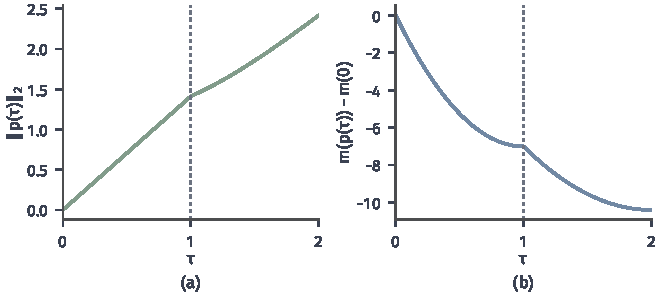
\includegraphics[width=112mm]{figures/05-optimization/02-smooth-optimization/matplotlib/tr-dogleg-monotone/figure.pdf}
 \caption{点$\bm{a}$的数据上沿狗腿路径的两个量，虚线$\tau=1$是折点$\bm{p}^{\mathrm{U}}$。(a)~长度严格增加。(b)~模型值严格减小。}
 \label{fig:tr-dogleg-monotone}
\end{BookInlineFigure}

\begin{lemma}[狗腿路径的单调性]
 \label{lem:tr-dogleg-monotone}
 设$\bm{B}\succ\bm{0}$，$\bm{g}\neq\bm{0}$。沿路径~\eqref{eq:tr-dogleg-path}，$\lVert\bm{p}(\tau)\rVert_2$单调不减，$m(\bm{p}(\tau))$单调不增。
\end{lemma}

\begin{proof}
 第一段上$\bm{p}$是从原点出发的线段，长度递增；$\bm{p}^{\mathrm{U}}$是模型沿这条射线的最小点，模型值递减。

 第二段记$\bm{w}=\bm{p}^{\mathrm{N}}-\bm{p}^{\mathrm{U}}$，$s=\tau-1\in[0,1]$。先看模型值。$h(s)=m(\bm{p}^{\mathrm{U}}+s\bm{w})$是凸二次函数，它在$s=1$处的导数是
 \[
  h'(1)=\langle\bm{B}\bm{p}^{\mathrm{N}}+\bm{g},\bm{w}\rangle=0,
 \]
 因为$\bm{B}\bm{p}^{\mathrm{N}}=-\bm{g}$。凸函数的导数单调不减，所以在$[0,1]$上$h'\leq0$。

 再看长度。$\tfrac12\lVert\bm{p}^{\mathrm{U}}+s\bm{w}\rVert_2^2$对$s$的导数是$\langle\bm{p}^{\mathrm{U}},\bm{w}\rangle+s\lVert\bm{w}\rVert_2^2$，只需证$\langle\bm{p}^{\mathrm{U}},\bm{w}\rangle\geq0$。记$\tau_{\mathrm{U}}>0$为式~\eqref{eq:tr-dogleg-points}中$\bm{g}$前的系数，代入该式，得到
 \[
  \langle\bm{p}^{\mathrm{U}},\bm{w}\rangle=\tau_{\mathrm{U}}\,\bm{g}^\top\bm{B}^{-1}\bm{g}-\tau_{\mathrm{U}}^2\,\bm{g}^\top\bm{g}
  =\frac{\tau_{\mathrm{U}}\bigl[(\bm{g}^\top\bm{B}^{-1}\bm{g})(\bm{g}^\top\bm{B}\bm{g})-(\bm{g}^\top\bm{g})^2\bigr]}{\bm{g}^\top\bm{B}\bm{g}}.
 \]
 取$\bm{u}=\bm{B}^{1/2}\bm{g}$，$\bm{v}=\bm{B}^{-1/2}\bm{g}$，方括号就是$\lVert\bm{u}\rVert_2^2\lVert\bm{v}\rVert_2^2-\langle\bm{u},\bm{v}\rangle^2$，由Cauchy--Schwarz不等式非负。
\end{proof}

\paragraph{计算过程}
下面用点$\bm{a}$的数据~\eqref{eq:tr-data-a}、半径$\Delta=2$走一遍。

需要的量是梯度$\bm{g}\in\mathbb{R}^n$、对称正定矩阵$\bm{B}\in\mathbb{R}^{n\times n}$、半径$\Delta$，输出位移$\bm{p}$。例中已知$\bm{g}=(7,7)^\top$，$\bm{B}=\operatorname{diag}(11,3)$。步骤如下。

\begin{enumerate}
 \item 由式~\eqref{eq:tr-dogleg-points}计算Newton点，若$\lVert\bm{p}^{\mathrm{N}}\rVert_2\leq\Delta$，返回$\bm{p}=\bm{p}^{\mathrm{N}}$。例中
 \[
  \bm{p}^{\mathrm{N}}=\begin{bmatrix}-7/11\\-7/3\end{bmatrix},\qquad\lVert\bm{p}^{\mathrm{N}}\rVert_2\approx2.419>2,
 \]
 所以继续。
 \item 由式~\eqref{eq:tr-dogleg-points}计算$\bm{p}^{\mathrm{U}}$，若$\lVert\bm{p}^{\mathrm{U}}\rVert_2\geq\Delta$，返回边界上的负梯度步$\bm{p}=-\Delta\bm{g}/\lVert\bm{g}\rVert_2$，这就是Cauchy步。例中
 \[
  \bm{p}^{\mathrm{U}}=-\frac{98}{686}\begin{bmatrix}7\\7\end{bmatrix}=\begin{bmatrix}-1\\-1\end{bmatrix},\qquad\lVert\bm{p}^{\mathrm{U}}\rVert_2=\sqrt2<2,
 \]
 所以继续。
 \item 否则交点在第二段上。记$\bm{w}=\bm{p}^{\mathrm{N}}-\bm{p}^{\mathrm{U}}$，解$\lVert\bm{p}^{\mathrm{U}}+s\bm{w}\rVert_2=\Delta$的正根：
 \begin{equation}
  s=\frac{-\langle\bm{p}^{\mathrm{U}},\bm{w}\rangle+\sqrt{\langle\bm{p}^{\mathrm{U}},\bm{w}\rangle^2+\lVert\bm{w}\rVert_2^2\bigl(\Delta^2-\lVert\bm{p}^{\mathrm{U}}\rVert_2^2\bigr)}}{\lVert\bm{w}\rVert_2^2}.
  \label{eq:tr-boundary-root}
 \end{equation}
 例中$\bm{w}=(4/11,\,-4/3)^\top$，三个系数是
 \[
  \lVert\bm{w}\rVert_2^2=\frac{2080}{1089},\qquad\langle\bm{p}^{\mathrm{U}},\bm{w}\rangle=\frac{1056}{1089},\qquad\Delta^2-\lVert\bm{p}^{\mathrm{U}}\rVert_2^2=2.
 \]
 根号内的量是$(2376/1089)^2$，因此
 \[
  s=\frac{-1056+2376}{2080}=\frac{33}{52}.
 \]
 \item 返回$\bm{p}=\bm{p}^{\mathrm{U}}+s\bm{w}$。例中
 \[
  \bm{p}=\begin{bmatrix}-1+3/13\\-1-11/13\end{bmatrix}=\begin{bmatrix}-10/13\\-24/13\end{bmatrix},
 \]
 长度恰为$\sqrt{100+576}/13=2$。
\end{enumerate}

最终得到的预测下降是
\[
 \operatorname{pred}(\bm{p})=\frac{238}{13}-\frac{1414}{169}=\frac{1680}{169}\approx9.941.
\]
这已经是全局解$10.115$的$98\%$，而全局解要解一元非线性方程。图~\ref{fig:tr-dogleg-path}给出三种半径下的结果：$\Delta=1$时只用到第一段，$\Delta=2$时落在第二段，$\Delta=3$时完整的Newton步被采用。

\begin{BookInlineFigure}
 \centering
 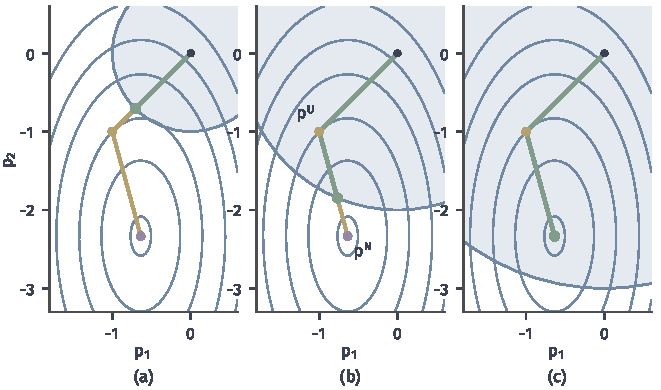
\includegraphics[width=112mm]{figures/05-optimization/02-smooth-optimization/matplotlib/tr-dogleg-path/figure.pdf}
 \caption{点$\bm{a}$的数据上半径分别为$1$、$2$、$3$的狗腿步。黄线是完整路径，绿线是实际走过的部分，绿点是得到的步。黄点是$\bm{p}^{\mathrm{U}}$，紫点是$\bm{p}^{\mathrm{N}}$，蓝线是模型等高线，浅蓝圆盘是信赖域。}
 \label{fig:tr-dogleg-path}
\end{BookInlineFigure}

狗腿步的预测下降不低于Cauchy步：若$\lVert\bm{p}^{\mathrm{U}}\rVert_2\geq\Delta$，两者相同；否则$\bm{p}^{\mathrm{U}}$本身就是Cauchy步，而由引理~\ref{lem:tr-dogleg-monotone}，狗腿步在路径上更靠后，模型值更低。所以它满足式~\eqref{eq:tr-sufficient-decrease}，$c_1=1/2$。

\paragraph{不正定时不能照搬}
上面的构造用到$\bm{B}\succ\bm{0}$：$\bm{p}^{\mathrm{N}}$要是模型的最小点，第二段上的模型才会下降。把原点的数据~\eqref{eq:tr-data-o}照搬进去，$\bm{g}^\top\bm{B}\bm{g}=2>0$，第一段还能算出$\bm{p}^{\mathrm{U}}=(-1,-1)^\top$，第二段却指向鞍点$(1,-1/3)^\top$。沿第二段模型上升，从$-1$一直升到$1/3$，图~\ref{fig:tr-dogleg-indefinite}画出了这一段。

\begin{BookInlineFigure}
 \centering
 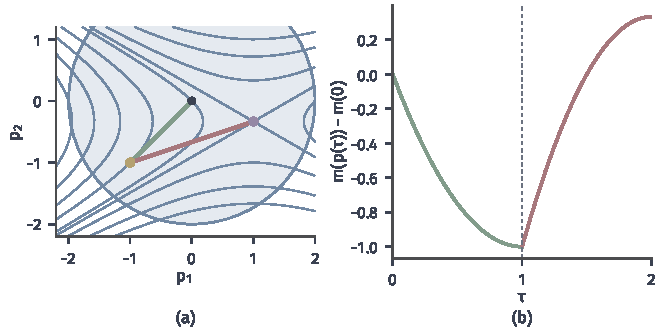
\includegraphics[width=112mm]{figures/05-optimization/02-smooth-optimization/matplotlib/tr-dogleg-indefinite/figure.pdf}
 \caption{把狗腿路径照搬到原点的不定模型上。(a)~模型等高线（蓝）与路径：绿色第一段走向黄点$\bm{p}^{\mathrm{U}}$，红色第二段走向模型的鞍点（紫）。(b)~沿路径的模型值，第二段（红）上升，路径上模型值的单调性失效。}
 \label{fig:tr-dogleg-indefinite}
\end{BookInlineFigure}

$\bm{B}$半正定且奇异时，$\bm{B}^{-1}$不存在，构造同样失效。这时要么先把$\bm{B}$修正成正定，要么换用下一小节的方法，后者不需要$\bm{B}$的任何分解。

\subsection{截断共轭梯度}
\label{sec:tr-truncated-cg}

\paragraph{主要思想}
Newton步是方程$\bm{B}\bm{p}=-\bm{g}$的解，也就是模型的驻点。第~\ref{chap:second-order-methods}章的Newton-CG用共轭梯度迭代近似解这个方程，只需要矩阵向量乘积。共轭梯度的推导和收敛性质可参考\BookChapterRef{chap:krylov-methods}{卷二第15章“Krylov子空间法”}，这里复述要用到的部分。

从$\bm{p}^{(0)}=\bm{0}$出发，记残差$\bm{r}^{(j)}=\bm{B}\bm{p}^{(j)}+\bm{g}$，它恰好是模型在$\bm{p}^{(j)}$处的梯度。内层迭代的上标用$j$，与外层的$t$区分。共轭梯度的递推是
\begin{equation}
 \begin{gathered}
  \alpha^{(j)}=\frac{\lVert\bm{r}^{(j)}\rVert_2^2}{\bm{d}^{(j)\top}\bm{B}\bm{d}^{(j)}},\qquad
  \bm{p}^{(j+1)}=\bm{p}^{(j)}+\alpha^{(j)}\bm{d}^{(j)},\\
  \bm{r}^{(j+1)}=\bm{r}^{(j)}+\alpha^{(j)}\bm{B}\bm{d}^{(j)},\\
  \beta^{(j)}=\frac{\lVert\bm{r}^{(j+1)}\rVert_2^2}{\lVert\bm{r}^{(j)}\rVert_2^2},\qquad
  \bm{d}^{(j+1)}=-\bm{r}^{(j+1)}+\beta^{(j)}\bm{d}^{(j)},
 \end{gathered}
 \label{eq:tr-cg}
\end{equation}
初始方向$\bm{d}^{(0)}=-\bm{g}$。$\alpha^{(j)}$是模型沿$\bm{d}^{(j)}$的精确一维最小点，所以每步模型值都下降。第一步恰好是$\bm{p}^{\mathrm{U}}$。

放进信赖域，只需要回答两个新问题：迭代走出半径了怎么办，遇到$\bm{B}$的非正曲率怎么办。\term{截断共轭梯度法}（truncated conjugate gradient method）的回答是：两种情况都沿当前方向走到边界，然后停止。

先看走出半径的情形。下面的引理说明，共轭梯度的迭代点离原点越来越远。一旦越出球，以后就不会回来，所以在第一次越界处截断不会错过后面的点。

\begin{lemma}[迭代点的长度递增]
 \label{lem:tr-cg-norm}
 设$\bm{g}\neq\bm{0}$，递推~\eqref{eq:tr-cg}进行到第$j$步，且此前各步曲率$\bm{d}^{(i)\top}\bm{B}\bm{d}^{(i)}>0$，残差非零。则
 \begin{equation}
  \lVert\bm{p}^{(j+1)}\rVert_2>\lVert\bm{p}^{(j)}\rVert_2.
  \label{eq:tr-cg-norm}
 \end{equation}
\end{lemma}

\begin{proof}
 残差相互正交，并且方向与残差张成同一子空间：
 \[
  \operatorname{span}\{\bm{d}^{(0)},\ldots,\bm{d}^{(j-1)}\}=\operatorname{span}\{\bm{r}^{(0)},\ldots,\bm{r}^{(j-1)}\}.
 \]
 这两条性质的归纳证明只用到递推~\eqref{eq:tr-cg}中的分母非零，不要求$\bm{B}$在全空间正定。由于$\bm{p}^{(j)}$是$\bm{d}^{(0)},\ldots,\bm{d}^{(j-1)}$的线性组合，所以$\langle\bm{p}^{(j)},\bm{r}^{(j)}\rangle=0$。

 用归纳法证明$\langle\bm{p}^{(j)},\bm{d}^{(j)}\rangle\geq0$。$j=0$时等于$0$。代入$\bm{d}^{(j+1)}$的定义，并用正交性，得到
 \[
  \langle\bm{p}^{(j+1)},\bm{d}^{(j+1)}\rangle=\beta^{(j)}\langle\bm{p}^{(j+1)},\bm{d}^{(j)}\rangle
  =\beta^{(j)}\bigl(\langle\bm{p}^{(j)},\bm{d}^{(j)}\rangle+\alpha^{(j)}\lVert\bm{d}^{(j)}\rVert_2^2\bigr),
 \]
 其中$\alpha^{(j)},\beta^{(j)}>0$，因此它非负。

 最后展开长度：
 \[
  \lVert\bm{p}^{(j+1)}\rVert_2^2=\lVert\bm{p}^{(j)}\rVert_2^2+2\alpha^{(j)}\langle\bm{p}^{(j)},\bm{d}^{(j)}\rangle+(\alpha^{(j)})^2\lVert\bm{d}^{(j)}\rVert_2^2>\lVert\bm{p}^{(j)}\rVert_2^2.
 \]
\end{proof}

再看非正曲率的情形。若$\bm{d}^{(j)\top}\bm{B}\bm{d}^{(j)}\leq0$，模型沿$\bm{d}^{(j)}$是凹的。由$\bm{r}^{(j)}$与$\bm{d}^{(j-1)}$正交可知模型沿$\bm{d}^{(j)}$的斜率为$-\lVert\bm{r}^{(j)}\rVert_2^2<0$，所以越往前走模型越低，应当一直走到边界。这正是第~\ref{sec:tr-model}节所说的利用负曲率。

三种停止各有含义，图~\ref{fig:tr-tcg-flow}是一步迭代的判断顺序。残差停止表示模型的驻点已经解得够准，判据沿用第~\ref{chap:second-order-methods}章非精确Newton法的形式：
\begin{equation}
 \lVert\bm{r}^{(j)}\rVert_2\leq\eta\lVert\bm{g}\rVert_2,\qquad\eta=\min\{0.1,\ \sqrt{\lVert\bm{g}\rVert_2}\}.
 \label{eq:tr-residual-stop}
\end{equation}

边界停止表示模型的最小点在球外。曲率停止表示模型沿这个方向没有最小点。后两条是信赖域给内层迭代新加的规则，Newton-CG遇到非正曲率时只能退回一个下降方向，交给线搜索。

\begin{BookInlineFigure}
 \centering
 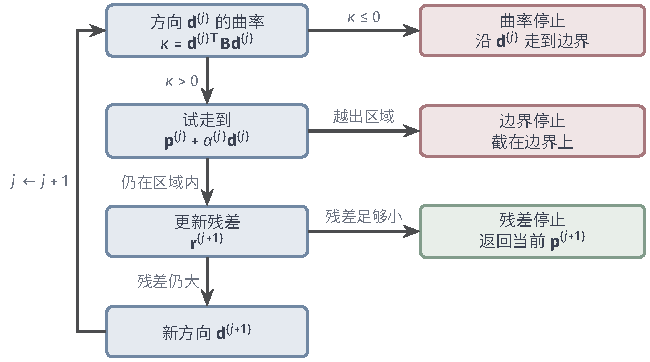
\includegraphics[width=110mm]{figures/05-optimization/02-smooth-optimization/tikz/tr-tcg-flow/figure.pdf}
 \caption{截断共轭梯度一次内层迭代的判断顺序。蓝框是普通的共轭梯度步骤，红框是信赖域带来的两种截断，绿框是沿用Newton-CG的残差停止。}
 \label{fig:tr-tcg-flow}
\end{BookInlineFigure}

\needspace{6\baselineskip}
\paragraph{变量}
下面的过程结合点$\bm{a}$的数据走一遍，要维护的量是：
\begin{itemize}
 \item $\bm{p}^{(j)}\in\mathbb{R}^n$：当前位移；
 \item $\bm{r}^{(j)}\in\mathbb{R}^n$：模型在$\bm{p}^{(j)}$处的梯度；
 \item $\bm{d}^{(j)}\in\mathbb{R}^n$：搜索方向；
 \item $\bm{B}\bm{d}^{(j)}\in\mathbb{R}^n$：一次矩阵向量乘积，是全部需要的曲率信息。
\end{itemize}

\paragraph{初始化}
取$\bm{p}^{(0)}=\bm{0}$，$\bm{r}^{(0)}=\bm{g}$，$\bm{d}^{(0)}=-\bm{g}$，容差$\eta$。例中半径$\Delta=2$，容差取$\eta=0.1$：
\[
 \bm{r}^{(0)}=\begin{bmatrix}7\\7\end{bmatrix},\qquad
 \bm{d}^{(0)}=\begin{bmatrix}-7\\-7\end{bmatrix},\qquad
 \eta\lVert\bm{g}\rVert_2\approx0.990.
\]

\paragraph{每轮更新}
第$j$轮依次执行以下步骤。

\begin{enumerate}
 \item 计算$\bm{B}\bm{d}^{(j)}$和曲率$\bm{d}^{(j)\top}\bm{B}\bm{d}^{(j)}$。若曲率不大于零，按式~\eqref{eq:tr-boundary-root}（其中$\bm{p}^{\mathrm{U}}$换成$\bm{p}^{(j)}$，$\bm{w}$换成$\bm{d}^{(j)}$）求出边界上的$\sigma$，返回$\bm{p}^{(j)}+\sigma\bm{d}^{(j)}$。例中第一轮
 \[
  \bm{B}\bm{d}^{(0)}=\begin{bmatrix}-77\\-21\end{bmatrix},\qquad
  \bm{d}^{(0)\top}\bm{B}\bm{d}^{(0)}=686>0.
 \]
 \item 由式~\eqref{eq:tr-cg}计算$\alpha^{(j)}$和试探点$\bm{p}^{(j)}+\alpha^{(j)}\bm{d}^{(j)}$。若试探点的长度不小于$\Delta$，同样求边界上的$\sigma$并返回。例中第一轮
 \[
  \alpha^{(0)}=\frac{98}{686}=\frac17,\qquad
  \bm{p}^{(1)}=\begin{bmatrix}-1\\-1\end{bmatrix},\qquad\lVert\bm{p}^{(1)}\rVert_2=\sqrt2<2.
 \]
 \item 由式~\eqref{eq:tr-cg}更新残差，若$\bm{r}^{(j+1)}$满足式~\eqref{eq:tr-residual-stop}，返回$\bm{p}^{(j+1)}$。例中第一轮
 \[
  \bm{r}^{(1)}=\begin{bmatrix}7\\7\end{bmatrix}+\frac17\begin{bmatrix}-77\\-21\end{bmatrix}=\begin{bmatrix}-4\\4\end{bmatrix},\qquad
  \lVert\bm{r}^{(1)}\rVert_2\approx5.66>0.990.
 \]
 \item 由式~\eqref{eq:tr-cg}计算$\beta^{(j)}$和新方向。例中第一轮
 \[
  \beta^{(0)}=\frac{32}{98}=\frac{16}{49},\qquad
  \bm{d}^{(1)}=\begin{bmatrix}4\\-4\end{bmatrix}+\frac{16}{49}\begin{bmatrix}-7\\-7\end{bmatrix}=\begin{bmatrix}12/7\\-44/7\end{bmatrix}.
 \]
\end{enumerate}

例中第二轮的曲率是
\[
 \bm{B}\bm{d}^{(1)}=\begin{bmatrix}132/7\\-132/7\end{bmatrix},\qquad
 \bm{d}^{(1)\top}\bm{B}\bm{d}^{(1)}=\frac{7392}{49}>0.
\]

于是$\alpha^{(1)}=32\cdot49/7392=7/33$。试探点正是Newton点，而它的长度约为$2.419$，超过了半径：
\[
 \bm{p}^{(1)}+\alpha^{(1)}\bm{d}^{(1)}=\begin{bmatrix}-7/11\\-7/3\end{bmatrix}.
\]

所以按边界停止。由式~\eqref{eq:tr-boundary-root}，边界上的$\sigma=7/52$，最终得到
\[
 \bm{p}=\begin{bmatrix}-1\\-1\end{bmatrix}+\frac{7}{52}\begin{bmatrix}12/7\\-44/7\end{bmatrix}=\begin{bmatrix}-10/13\\-24/13\end{bmatrix}.
\]

这和狗腿步完全相同，并不是巧合。二维时共轭梯度第一步到$\bm{p}^{\mathrm{U}}$，第二步到$\bm{p}^{\mathrm{N}}$，两段路径就是狗腿路径。维数大于$2$时两者不同：狗腿法从$\bm{p}^{\mathrm{U}}$直奔Newton点，截断共轭梯度沿途经过一串中间点，也不需要预先分解$\bm{B}$。半径若取$\Delta=3$，第二轮的试探点在球内，残差恰好为零，按残差停止，返回Newton步。

再用原点的数据~\eqref{eq:tr-data-o}、$\Delta=2$看曲率停止。第一轮的曲率$\bm{d}^{(0)\top}\bm{B}\bm{d}^{(0)}=2>0$，$\alpha^{(0)}=1$，试探点在球内，并有
\[
 \bm{p}^{(1)}=\begin{bmatrix}-1\\-1\end{bmatrix},\qquad
 \bm{r}^{(1)}=\begin{bmatrix}2\\-2\end{bmatrix},\qquad
 \bm{d}^{(1)}=\begin{bmatrix}-6\\-2\end{bmatrix}.
\]

第二轮的曲率是$-36+12=-24\leq0$，沿$\bm{d}^{(1)}$走到边界。由$\lVert\bm{p}^{(1)}+\sigma\bm{d}^{(1)}\rVert_2=2$得$20\sigma^2+8\sigma-1=0$，取正根$\sigma=1/10$，最终得到
\[
 \bm{p}=\begin{bmatrix}-8/5\\-6/5\end{bmatrix},\qquad\operatorname{pred}(\bm{p})=\frac{48}{25}=1.92.
\]
图~\ref{fig:tr-tcg-path}是这两次运行的轨迹。

\begin{BookInlineFigure}
 \centering
 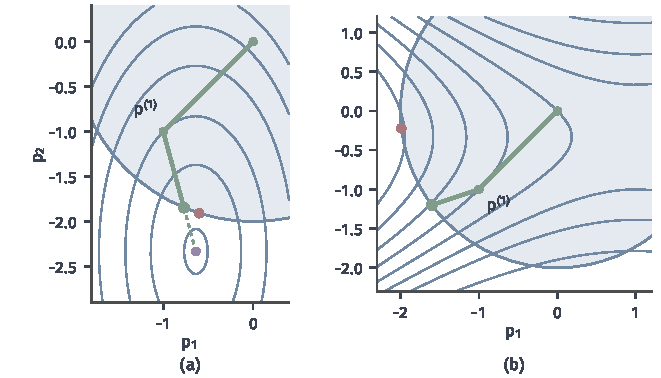
\includegraphics[width=112mm]{figures/05-optimization/02-smooth-optimization/matplotlib/tr-tcg-path/figure.pdf}
 \caption{截断共轭梯度的两次运行，绿线是迭代轨迹，绿色大点是返回的步，红点是子问题的全局解。(a)~点$\bm{a}$，第二轮越过边界而截断，虚线通向球外的Newton点（紫）。(b)~原点，第二轮遇到负曲率，沿方向走到边界。}
 \label{fig:tr-tcg-path}
\end{BookInlineFigure}

\paragraph{算法分析}
截断共轭梯度的第一轮要么到达$\bm{p}^{\mathrm{U}}$，要么在边界上截断，得到的都是Cauchy步，此后每一步模型值都不升高：普通步是精确一维最小化，边界截断发生在模型仍然下降的路段上。所以它的预测下降不低于Cauchy步，满足式~\eqref{eq:tr-sufficient-decrease}，$c_1=1/2$。

当$\bm{B}\succ\bm{0}$时还可以证明，截断共轭梯度的预测下降至少是全局解的一半，证明需要细致比较Krylov子空间上的子问题，篇幅较长，读者可查阅专门的信赖域文献。$\bm{B}$不定时没有这个保证：原点上它的预测下降只有$1.92$，全局解是$4.111$。它在图~\ref{fig:tr-tcg-path}(b)中沿方向$(-3,-1)^\top$走到边界，错过了曲率最负的方向$\bm{e}_1$。

表~\ref{tab:tr-subproblem-compare}汇总同一个模型上三种步和全局解的结果。

\begin{BookInlineTable}
 \centering
 \begin{tabular}{llrrrr}
  \toprule
  模型 & 量 & Cauchy步 & 狗腿步 & 截断共轭梯度 & 全局解\\
  \midrule
  点$\bm{a}$ & $\operatorname{pred}$ & $7.000$ & $9.941$ & $9.941$ & $10.115$\\
  & $\operatorname{ared}$ & $8.750$ & $10.764$ & $10.764$ & $10.515$\\
  原点 & $\operatorname{pred}$ & $1.000$ & 不适用 & $1.920$ & $4.111$\\
  & $\operatorname{ared}$ & $0.750$ & 不适用 & $0.282$ & $0.209$\\
  \bottomrule
 \end{tabular}
 \caption{半径$\Delta=2$时几种步的预测下降与实际下降。}
 \label{tab:tr-subproblem-compare}
\end{BookInlineTable}

二维例子看不出截断共轭梯度的省力之处。图~\ref{fig:tr-tcg-compare}取一个$n=200$的正定模型：Hessian向量乘积只用$9$次，预测下降就达到全局解的$98\%$，长度随次数严格增加，与引理~\ref{lem:tr-cg-norm}一致。这时狗腿法和精确求解都要作$200$阶矩阵的分解。

\begin{BookInlineFigure}
 \centering
 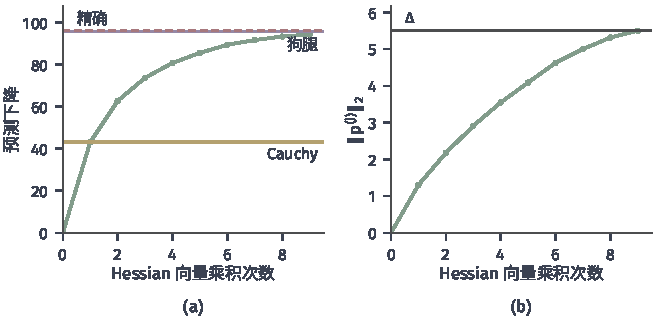
\includegraphics[width=112mm]{figures/05-optimization/02-smooth-optimization/matplotlib/tr-tcg-compare/figure.pdf}
 \caption{一个$n=200$的随机正定模型，特征值在$1$到$100$之间对数等距，$\Delta=5.5$，随机种子固定。(a)~截断共轭梯度（绿）的预测下降随矩阵向量乘积次数的变化，水平线依次为Cauchy步（黄）、狗腿步（紫）和全局解（红虚线）。(b)~迭代点长度（绿）递增，触及半径（深灰线）时停止。}
 \label{fig:tr-tcg-compare}
\end{BookInlineFigure}

\section{步的接受与半径更新}
\label{sec:tr-acceptance}

子问题给出了一个候选步，但模型的话不能全信。这就需要回答：怎样用真实目标检验这一步，并决定下一轮用多大的半径？

\paragraph{主要思想}
第~\ref{sec:tr-model}节已经分开了预测下降和实际下降，把它们相除就是一个无量纲的检验量。定义\term{下降比}（reduction ratio）：
\begin{equation}
 \rho^{(t)}=\frac{\operatorname{ared}(\bm{p}^{(t)})}{\operatorname{pred}(\bm{p}^{(t)})}
 =\frac{f(\bm{x}^{(t)})-f(\bm{x}^{(t)}+\bm{p}^{(t)})}{m^{(t)}(\bm{0})-m^{(t)}(\bm{p}^{(t)})}.
 \label{eq:tr-rho}
\end{equation}
只要$\bm{g}^{(t)}\neq\bm{0}$且候选步满足式~\eqref{eq:tr-sufficient-decrease}，分母就为正，比值有意义。

$\rho^{(t)}$接近$1$，说明模型在这个范围内预测得准。$\rho^{(t)}$是很小的正数，说明目标虽有下降，但比预测差得多。$\rho^{(t)}$为负，说明目标实际上升了。$\rho^{(t)}$大于$1$，说明目标比模型预测的下降更多，这是好事，但也表明模型并不精确。

用两个阈值$0<\eta_1\leq\eta_2<1$把数轴分成三段，常取$\eta_1=1/4$，$\eta_2=3/4$；另取缩小因子$\theta\in(0,1)$和半径上限$\Delta_{\max}$。下一个点按是否接受决定：
\begin{equation}
 \bm{x}^{(t+1)}=
 \begin{cases}
  \bm{x}^{(t)}+\bm{p}^{(t)},&\rho^{(t)}\geq\eta_1,\\
  \bm{x}^{(t)},&\rho^{(t)}<\eta_1.
 \end{cases}
 \label{eq:tr-accept}
\end{equation}

下一轮的半径按模型的表现决定：
\begin{equation}
 \Delta^{(t+1)}=
 \begin{cases}
  \theta\Delta^{(t)},&\rho^{(t)}<\eta_1,\\
  \min\{2\Delta^{(t)},\Delta_{\max}\},&\rho^{(t)}\geq\eta_2\text{ 且步在边界},\\
  \Delta^{(t)},&\text{其他情形}.
 \end{cases}
 \label{eq:tr-radius}
\end{equation}

第二种情形多了“步在边界”这个条件，即$\lVert\bm{p}^{(t)}\rVert_2=\Delta^{(t)}$：若步在球内部，半径并没有限制住它，扩大半径没有意义。图~\ref{fig:tr-rho-decision}把这三段画在数轴上。

\begin{BookInlineFigure}
 \centering
 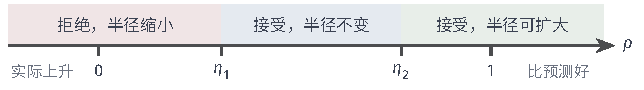
\includegraphics[width=109mm]{figures/05-optimization/02-smooth-optimization/tikz/tr-rho-decision/figure.pdf}
 \caption{下降比$\rho$的三段及相应动作。红色段拒绝这一步，蓝色段接受但半径不变，绿色段接受，并且在步到达边界时扩大半径。}
 \label{fig:tr-rho-decision}
\end{BookInlineFigure}

拒绝一步的代价比看上去小。点没有动，梯度和$\bm{B}$都不用重算，下一轮用同一个模型在更小的球里重解子问题。这里要与线搜索的回溯对比：回溯只缩短长度，方向不变；信赖域缩小半径后，新的解方向一般也变了。图~\ref{fig:tr-loop}是完整的一轮。

\begin{BookInlineFigure}
 \centering
 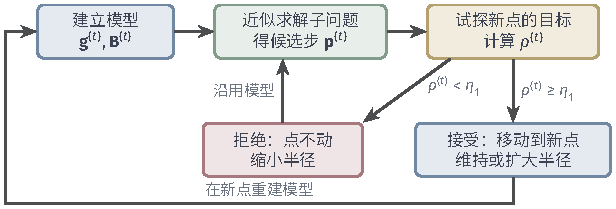
\includegraphics[width=104mm]{figures/05-optimization/02-smooth-optimization/tikz/tr-loop/figure.pdf}
 \caption{信赖域方法的一轮。黄框里的目标值是这一轮唯一一次新增的函数值计算。接受时回到左侧在新点重建模型，拒绝时模型沿用，只在更小的球内重解子问题。}
 \label{fig:tr-loop}
\end{BookInlineFigure}

\paragraph{模型矩阵从哪里来}
框架对$\bm{B}^{(t)}$的要求很少：对称，范数有界。取Hessian得到信赖域Newton法；取第~\ref{chap:quasi-newton}章的BFGS近似也可以。第~\ref{chap:quasi-newton}章的SR1更新尤其适合这里，它由位移$\bm{s}=\bm{p}^{(t)}$和梯度差$\bm{y}$得到
\begin{equation}
 \bm{B}^{(t+1)}=\bm{B}^{(t)}+\frac{(\bm{y}-\bm{B}^{(t)}\bm{s})(\bm{y}-\bm{B}^{(t)}\bm{s})^\top}{\langle\bm{y}-\bm{B}^{(t)}\bm{s},\bm{s}\rangle}.
 \label{eq:tr-sr1}
\end{equation}

SR1不保持正定性，$\bm{B}^{(t+1)}$可能不定，放进线搜索框架时方向可能不是下降方向，这在信赖域中不成问题。分母过小时跳过更新。即使这一步被拒绝，$\bm{s}$和$\bm{y}$仍然是真实的曲率信息，通常也用来更新，代价是在试探点多算一次梯度。这时$\bm{B}^{(t)}$已不是$\bm{H}^{(t)}$，下面的手算例子仍用Hessian。

\needspace{6\baselineskip}
\paragraph{变量}
下面用目标~\eqref{eq:tr-example}走完整个过程，子问题用截断共轭梯度求解。要维护的量是：
\begin{itemize}
 \item $\bm{x}^{(t)}\in\mathbb{R}^n$：当前点，$f(\bm{x}^{(t)})$是它的目标值；
 \item $\Delta^{(t)}>0$：当前半径；
 \item $\bm{g}^{(t)}\in\mathbb{R}^n$，$\bm{B}^{(t)}\in\mathbb{R}^{n\times n}$：当前模型，上一轮被拒绝时直接沿用。
\end{itemize}

\paragraph{初始化}
选定$\bm{x}^{(0)}$，$\Delta^{(0)}$，阈值和缩小因子。例中取
\[
 \bm{x}^{(0)}=\begin{bmatrix}0\\0\end{bmatrix},\qquad\Delta^{(0)}=2,\qquad\Delta_{\max}=8,
\]
\[
 \eta_1=\frac14,\qquad\eta_2=\frac34,\qquad\theta=\frac12.
\]

\paragraph{每轮更新}
第$t$轮依次执行以下步骤，直到$\lVert\bm{g}^{(t)}\rVert_2$小于给定的容差。

\begin{enumerate}
 \item 若上一轮接受了步，由式~\eqref{eq:tr-example-derivatives}计算$\bm{g}^{(t)}$和$\bm{B}^{(t)}$。例中第$0$轮得到数据~\eqref{eq:tr-data-o}。
 \item 近似求解子问题~\eqref{eq:tr-subproblem}，得到$\bm{p}^{(t)}$。例中第$0$轮就是上一节算过的曲率停止：
 \[
  \bm{p}^{(0)}=\begin{bmatrix}-1.6\\-1.2\end{bmatrix},\qquad\operatorname{pred}(\bm{p}^{(0)})=1.92.
 \]
 \item 由式~\eqref{eq:tr-rho}计算$\rho^{(t)}$。例中第$0$轮由式~\eqref{eq:tr-example-error}，模型误差是$\tfrac14(1.6)^4=1.6384$，于是
 \[
  \operatorname{ared}(\bm{p}^{(0)})=1.92-1.6384=0.2816,\qquad\rho^{(0)}\approx0.147.
 \]
 \item 由式~\eqref{eq:tr-accept}和式~\eqref{eq:tr-radius}决定下一个点和半径。例中第$0$轮$\rho^{(0)}<1/4$，拒绝这一步，并有
 \[
  \bm{x}^{(1)}=\begin{bmatrix}0\\0\end{bmatrix},\qquad\Delta^{(1)}=1.
 \]
\end{enumerate}

第$1$轮沿用同一个模型。半径变成$1$，共轭梯度的第一步$(-1,-1)^\top$长度为$\sqrt2$，已越过边界，所以截断在球面上：
\[
 \bm{p}^{(1)}=\begin{bmatrix}-1/\sqrt2\\-1/\sqrt2\end{bmatrix},\qquad\operatorname{pred}(\bm{p}^{(1)})=\sqrt2-\frac12\approx0.9142.
\]

模型误差是$\tfrac14(1/\sqrt2)^4=0.0625$，于是实际下降约为$0.8517$，比值$\rho^{(1)}\approx0.932\geq3/4$。这一步在边界上，接受并把半径扩大：
\[
 \bm{x}^{(2)}\approx\begin{bmatrix}-0.7071\\-0.7071\end{bmatrix},\qquad\Delta^{(2)}=2.
\]
半径减半之后，步的方向由$(-1.6,-1.2)$变成了负梯度方向，这正是前面说的方向随半径变化。图~\ref{fig:tr-rejection}把这两次试探画在真实目标上。

\begin{BookInlineFigure}
 \centering
 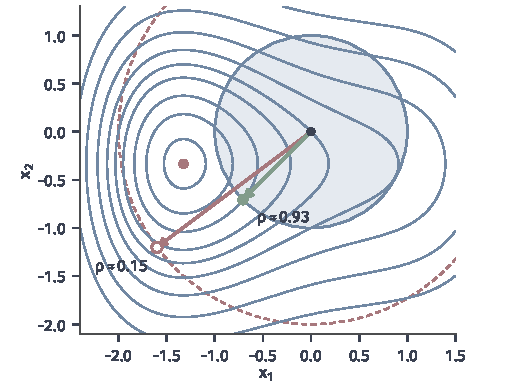
\includegraphics[width=90mm]{figures/05-optimization/02-smooth-optimization/matplotlib/tr-rejection/figure.pdf}
 \caption{原点处的一次拒绝与一次接受，蓝线是目标~\eqref{eq:tr-example}的等高线。红色虚线圆和红色箭头是$\Delta=2$的试探，空心点被拒绝；浅蓝圆盘和绿色箭头是$\Delta=1$的试探，绿点被接受。红色实心点是最小点。}
 \label{fig:tr-rejection}
\end{BookInlineFigure}

第$2$轮由式~\eqref{eq:tr-example-derivatives}重建模型：
\[
 \bm{g}^{(2)}\approx\begin{bmatrix}1.3536\\-1.1213\end{bmatrix},\qquad\bm{B}^{(2)}\approx\begin{bmatrix}0.5&0\\0&3\end{bmatrix}.
\]

这时$\bm{B}$已经正定，但$x_1$方向的曲率只有$0.5$，比前方实际的曲率小得多。$\Delta=2$的步是$\bm{p}^{(2)}\approx(-1.928,0.530)^\top$，预测下降$1.853$，实际却上升$6.674$，$\rho^{(2)}\approx-3.60$，又被拒绝。第$3$轮半径减半后，比值回到$0.589$，接受，半径保持为$1$。

继续下去，第$4$轮开始Newton步已落在球内，由残差停止，半径不再起作用，比值接近$1$，梯度范数迅速下降。表~\ref{tab:tr-history}列出全部$8$轮，最终得到$\bm{x}\approx(-1.3247,-0.3333)^\top$，$f\approx-1.5989$，这就是$\bm{x}^\star$。图~\ref{fig:tr-outer-path}是轨迹和半径的变化。

\begin{BookInlineTable}
 \centering
 \begin{tabular}{rrrcrrrl}
  \toprule
  $t$ & $f(\bm{x}^{(t)})$ & $\Delta^{(t)}$ & 停止 & pred & ared & $\rho^{(t)}$ & 结果\\
  \midrule
  $0$ & $0.000$ & $2$ & 曲率 & $1.920$ & $0.282$ & $0.147$ & 拒绝\\
  $1$ & $0.000$ & $1$ & 边界 & $0.914$ & $0.852$ & $0.932$ & 接受，扩大\\
  $2$ & $-0.852$ & $2$ & 边界 & $1.853$ & $-6.674$ & $-3.602$ & 拒绝\\
  $3$ & $-0.852$ & $1$ & 边界 & $0.999$ & $0.588$ & $0.589$ & 接受\\
  $4$ & $-1.440$ & $1$ & 残差 & $0.155$ & $0.158$ & $1.023$ & 接受\\
  $5$ & $-1.598$ & $1$ & 残差 & $0.001$ & $0.001$ & $1.011$ & 接受\\
  $6$ & $-1.599$ & $1$ & 残差 & $0.000$ & $0.000$ & $1.000$ & 接受\\
  $7$ & $-1.599$ & $1$ & 残差 & $0.000$ & $0.000$ & $0.999$ & 接受\\
  \bottomrule
 \end{tabular}
 \caption{贯穿例子的完整运行。pred和ared是预测下降与实际下降，“停止”是内层截断共轭梯度的停止原因。}
 \label{tab:tr-history}
\end{BookInlineTable}

\begin{BookInlineFigure}
 \centering
 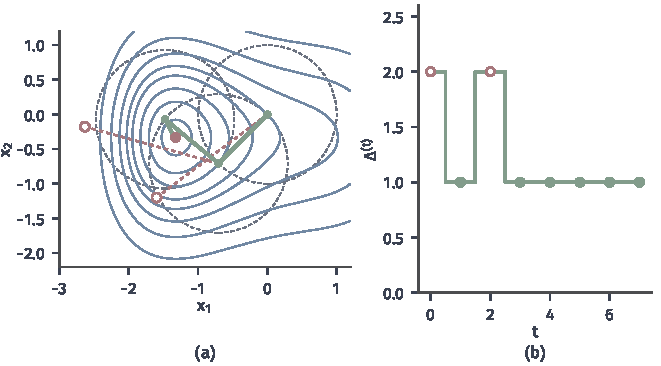
\includegraphics[width=112mm]{figures/05-optimization/02-smooth-optimization/matplotlib/tr-outer-path/figure.pdf}
 \caption{贯穿例子的完整运行。(a)~目标等高线（蓝）上的轨迹（绿），虚线圆是前几轮被接受时的信赖域，红色虚线和空心点是被拒绝的试探，红点是最小点。(b)~半径随轮数的变化，实心点表示接受，空心点表示拒绝。}
 \label{fig:tr-outer-path}
\end{BookInlineFigure}

这次运行显示了框架的分工：远离解时，半径起主导作用，负责把模型限制在可信的范围；靠近解时，半径不再起作用，方法退化成普通的Newton法。半径的调整不需要人工干预，由下降比自动完成。

\section{收敛与计算成本}
\label{sec:tr-convergence}

前几节的例子看起来都收敛了，在什么条件下这是必然的，极限点是什么样的点，每一轮又要花多少计算？

\paragraph{假设}
一阶结果需要下面三条假设。
\begin{enumerate}
 \item $f$连续可微，下有界，$f\geq f_{\mathrm{low}}$，梯度在$\mathbb{R}^n$上Lipschitz连续，常数为$L$。
 \item 模型矩阵一致有界：$\bm{B}^{(t)}$对称，$\lVert\bm{B}^{(t)}\rVert_2\leq M$，$M>0$。
 \item 候选步可行，$\lVert\bm{p}^{(t)}\rVert_2\leq\Delta^{(t)}$，并且对某个$c_1\in(0,1]$满足充分模型下降：
 \begin{equation}
  \operatorname{pred}(\bm{p}^{(t)})\geq c_1\lVert\bm{g}^{(t)}\rVert_2\min\Bigl\{\Delta^{(t)},\ \frac{\lVert\bm{g}^{(t)}\rVert_2}{M}\Bigr\}.
  \label{eq:tr-assumption-decrease}
 \end{equation}
\end{enumerate}

第三条由式~\eqref{eq:tr-sufficient-decrease}和$\lVert\bm{B}^{(t)}\rVert_2\leq M$推出，前面三种求解器都满足。第一条的全局Lipschitz条件可以放宽：目标~\eqref{eq:tr-example}的梯度不是全局Lipschitz的，但它的水平集有界，半径又有上限$\Delta_{\max}$，试探点都落在一个紧集内，$L$只需在这个紧集上成立。

条件里没有要求$\bm{B}^{(t)}$接近Hessian，也没有要求子问题解得精确。模型只要在一阶上与目标匹配，这正是拟牛顿模型能够进入这个框架的原因。

\paragraph{半径不会塌缩}
证明的核心是一个观察：半径足够小时，模型误差相对预测下降可以忽略，这一步一定被接受。模型误差是半径的二次量，预测下降却是半径的一次量，两者之比随半径趋于零。图~\ref{fig:tr-radius-rho}在点$\bm{a}$上验证了这一点：取精确Hessian时$\lvert1-\rho\rvert$随半径的斜率是$2$，取粗糙的$\bm{B}=\bm{I}$时斜率是$1$，后者正是定理使用的一般界。

\begin{BookInlineFigure}
 \centering
 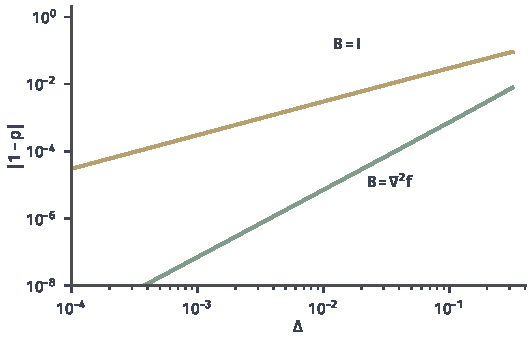
\includegraphics[width=90mm]{figures/05-optimization/02-smooth-optimization/matplotlib/tr-radius-rho/figure.pdf}
 \caption{在点$\bm{a}$沿负梯度方向取长度$\Delta$的步，$\lvert1-\rho\rvert$随$\Delta$的变化（对数坐标）。绿线的模型矩阵是Hessian，斜率约为$2$；黄线的模型矩阵是$\bm{I}$，斜率约为$1$。两条线都随$\Delta\to0$趋于零。}
 \label{fig:tr-radius-rho}
\end{BookInlineFigure}

\begin{theorem}[梯度的下极限为零]
 \label{thm:tr-first-order}
 在上述三条假设下，设外层迭代按式~\eqref{eq:tr-accept}和式~\eqref{eq:tr-radius}更新，其中$\eta_1>0$。此时
 \begin{equation}
  \liminf_{t\to\infty}\lVert\bm{g}^{(t)}\rVert_2=0.
  \label{eq:tr-liminf}
 \end{equation}
\end{theorem}

\begin{proof}
 反设存在$\varepsilon>0$和$T_0$，使得$t\geq T_0$时$\lVert\bm{g}^{(t)}\rVert_2\geq\varepsilon$。

 第一步估计模型误差。由梯度Lipschitz连续，对任意$\bm{p}$，
 \[
  \bigl\lvert f(\bm{x}+\bm{p})-f(\bm{x})-\langle\bm{g},\bm{p}\rangle\bigr\rvert
  =\Bigl\lvert\int_0^1\langle\nabla f(\bm{x}+s\bm{p})-\bm{g},\bm{p}\rangle\,\mathrm{d}s\Bigr\rvert
  \leq\frac{L}{2}\lVert\bm{p}\rVert_2^2.
 \]
 再计入模型的二次项，且$\lVert\bm{p}^{(t)}\rVert_2\leq\Delta^{(t)}$，得到
 \[
  \bigl\lvert f(\bm{x}^{(t)}+\bm{p}^{(t)})-m^{(t)}(\bm{p}^{(t)})\bigr\rvert\leq\frac{L+M}{2}(\Delta^{(t)})^2.
 \]

 第二步说明小半径时不会缩小。令
 \[
  K=\min\Bigl\{\frac1M,\ \frac{2c_1(1-\eta_2)}{L+M}\Bigr\}.
 \]
 设$t\geq T_0$且$\Delta^{(t)}\leq K\varepsilon$。此时$\Delta^{(t)}\leq\varepsilon/M$，不超过$\lVert\bm{g}^{(t)}\rVert_2/M$，所以式~\eqref{eq:tr-assumption-decrease}的最小值取在$\Delta^{(t)}$上：
 \[
  \operatorname{pred}(\bm{p}^{(t)})\geq c_1\varepsilon\Delta^{(t)}.
 \]
 又$m^{(t)}(\bm{0})=f(\bm{x}^{(t)})$，所以预测下降与实际下降之差就是模型误差，于是
 \[
  \lvert1-\rho^{(t)}\rvert\leq\frac{(L+M)(\Delta^{(t)})^2/2}{c_1\varepsilon\Delta^{(t)}}=\frac{(L+M)\Delta^{(t)}}{2c_1\varepsilon}\leq1-\eta_2.
 \]
 因此$\rho^{(t)}\geq\eta_2\geq\eta_1$，这一轮半径不缩小。

 第三步得到半径的下界。半径只在$\Delta^{(t)}>K\varepsilon$时才可能缩小，缩小后不低于$\theta K\varepsilon$，所以对$t\geq T_0$，
 \[
  \Delta^{(t)}\geq\Delta_{\min}:=\min\{\Delta^{(T_0)},\ \theta K\varepsilon\}>0.
 \]

 第四步导出矛盾。若被接受的轮只有有限多次，则此后点不动，半径每轮乘以$\theta$，趋于零，与下界矛盾。所以接受无穷多次，每次接受时$\rho^{(t)}\geq\eta_1$，并由式~\eqref{eq:tr-assumption-decrease}，
 \[
  f(\bm{x}^{(t)})-f(\bm{x}^{(t+1)})\geq\eta_1\operatorname{pred}(\bm{p}^{(t)})
  \geq\eta_1c_1\varepsilon\min\Bigl\{\Delta_{\min},\ \frac{\varepsilon}{M}\Bigr\}>0.
 \]
 目标值单调不增，却无穷多次下降一个固定的量，这与$f\geq f_{\mathrm{low}}$矛盾。
\end{proof}

下极限只说明有一个子列的梯度趋于零。$\eta_1>0$时可以加强：整个序列的梯度都趋于零。

\begin{theorem}[梯度趋于零]
 \label{thm:tr-limit}
 在定理~\ref{thm:tr-first-order}的条件下，
 \begin{equation}
  \lim_{t\to\infty}\lVert\bm{g}^{(t)}\rVert_2=0.
  \label{eq:tr-limit}
 \end{equation}
\end{theorem}

\begin{proof}
 反设存在$\varepsilon>0$和无穷多个下标$t$满足$\lVert\bm{g}^{(t)}\rVert_2\geq2\varepsilon$。对每个这样的$t$，由定理~\ref{thm:tr-first-order}，存在最小的$l(t)>t$使$\lVert\bm{g}^{(l(t))}\rVert_2<\varepsilon$。在$t\leq k<l(t)$的轮中$\lVert\bm{g}^{(k)}\rVert_2\geq\varepsilon$。记其中被接受的轮的集合为$\mathcal{K}$。

 由Lipschitz条件和$\lVert\bm{p}^{(k)}\rVert_2\leq\Delta^{(k)}$，这段路程的总长度不能太短：
 \[
  \varepsilon\leq\lVert\bm{g}^{(t)}\rVert_2-\lVert\bm{g}^{(l(t))}\rVert_2\leq L\sum_{k\in\mathcal{K}}\lVert\bm{p}^{(k)}\rVert_2\leq L\sum_{k\in\mathcal{K}}\Delta^{(k)}.
 \]

 这段路程上目标的下降量由接受规则和式~\eqref{eq:tr-assumption-decrease}控制：
 \[
  f(\bm{x}^{(t)})-f(\bm{x}^{(l(t))})\geq\eta_1c_1\varepsilon\sum_{k\in\mathcal{K}}\min\Bigl\{\Delta^{(k)},\ \frac{\varepsilon}{M}\Bigr\}.
 \]

 若$\mathcal{K}$中某一项有$\Delta^{(k)}>\varepsilon/M$，右端至少是$\eta_1c_1\varepsilon^2/M$。否则右端等于$\eta_1c_1\varepsilon\sum\Delta^{(k)}$，至少是$\eta_1c_1\varepsilon^2/L$。两种情形下降量都有一个不依赖$t$的正下界。但$f(\bm{x}^{(t)})$单调且有下界，$t\to\infty$时$f(\bm{x}^{(t)})-f(\bm{x}^{(l(t))})\to0$，矛盾。
\end{proof}

条件的作用可以逐条核对。去掉下有界，目标可以一直下降，例如$f(x)=-x$，梯度恒为$-1$。去掉$\eta_1>0$的接受门槛，只要求$\rho^{(t)}>0$，下降量可以任意小，一般只能得到下极限的结论。去掉充分模型下降，候选步可以小到没有进展，比值$\rho^{(t)}$即使接近$1$也无济于事。

\paragraph{二阶保证}
定理~\ref{thm:tr-limit}只说明极限点是驻点，鞍点也是驻点。要排除负曲率，候选步必须真正使用负曲率。设$\bm{B}^{(t)}=\bm{H}^{(t)}$，用下面的量衡量负曲率的大小：
\[
 \lambda^{(t)}_-=\max\{0,\ -\lambda_{\min}(\bm{H}^{(t)})\}.
\]
要求存在常数$c_2>0$，使得
\begin{equation}
 \operatorname{pred}(\bm{p}^{(t)})\geq c_2\lambda^{(t)}_-(\Delta^{(t)})^2.
 \label{eq:tr-eigen-decrease}
\end{equation}

子问题的全局解满足这一条，$c_2=1/2$。取$\bm{u}$是$\lambda_{\min}$的单位特征向量，选符号使$\langle\bm{g},\bm{u}\rangle\leq0$，点$\Delta\bm{u}$可行，由它的模型值得
\[
 m(\bm{0})-m(\Delta\bm{u})=-\Delta\langle\bm{g},\bm{u}\rangle-\frac12\lambda_{\min}\Delta^2\geq\frac12\lambda_-\Delta^2,
\]
全局解的预测下降不低于这个量。

Cauchy步和截断共轭梯度不满足式~\eqref{eq:tr-eigen-decrease}。第~\ref{sec:tr-model}节困难情形的数据$\bm{g}=(0,1)^\top$，$\bm{B}=\operatorname{diag}(-1,3)$，$\Delta=1$就是反例。截断共轭梯度第一步$\bm{d}^{(0)}=(0,-1)^\top$，曲率为正，一步到$(0,-1/3)^\top$，残差为零而停止，预测下降只有$1/6$。全局解的预测下降是$5/8$，并且沿$\bm{e}_1$方向使用了负曲率。迭代只在Krylov子空间中进行，而这个子空间恰好与$\bm{e}_1$正交，图~\ref{fig:tr-second-order}(a)画出了这一点。若$\bm{g}=\bm{0}$，迭代第一步就停在$\bm{p}=\bm{0}$，负曲率完全看不到。

\begin{theorem}[二阶下极限]
 \label{thm:tr-second-order}
 在定理~\ref{thm:tr-first-order}的条件之外，设$\bm{B}^{(t)}=\bm{H}^{(t)}$，Hessian是$L_H$-Lipschitz的，且候选步满足式~\eqref{eq:tr-eigen-decrease}。则
 \begin{equation}
  \liminf_{t\to\infty}\max\bigl\{\lVert\bm{g}^{(t)}\rVert_2,\ \lambda^{(t)}_-\bigr\}=0.
  \label{eq:tr-second-order}
 \end{equation}
\end{theorem}

\begin{proof}
 反设存在$\varepsilon>0$和$T_0$，使得$t\geq T_0$时
 \[
  \max\{\lVert\bm{g}^{(t)}\rVert_2,\ \lambda^{(t)}_-\}\geq\varepsilon.
 \]
 若$\lVert\bm{g}^{(t)}\rVert_2\geq\varepsilon$，定理~\ref{thm:tr-first-order}证明的第二步依然适用。若$\lambda^{(t)}_-\geq\varepsilon$，由Hessian的Lipschitz条件，模型误差不超过$L_H\lVert\bm{p}\rVert_2^3/6$，再用式~\eqref{eq:tr-eigen-decrease}，
 \[
  \lvert1-\rho^{(t)}\rvert\leq\frac{L_H(\Delta^{(t)})^3/6}{c_2\varepsilon(\Delta^{(t)})^2}=\frac{L_H\Delta^{(t)}}{6c_2\varepsilon}.
 \]
 所以取$K_2=\min\{K,\ 6c_2(1-\eta_2)/L_H\}$，$\Delta^{(t)}\leq K_2\varepsilon$时半径不缩小，同样得到半径的正下界$\Delta_{\min}$。每次接受至少下降
 \[
  \eta_1\min\Bigl\{c_1\varepsilon\min\bigl\{\Delta_{\min},\ \varepsilon/M\bigr\},\ c_2\varepsilon\Delta_{\min}^2\Bigr\}>0,
 \]
 与定理~\ref{thm:tr-first-order}证明的第四步一样导出矛盾。
\end{proof}

这个定理给出的是一个子列上的结论：若该子列有极限点$\bar{\bm{x}}$，则$\nabla f(\bar{\bm{x}})=\bm{0}$且$\nabla^2f(\bar{\bm{x}})\succeq\bm{0}$。这只是二阶必要条件，并不说明$\bar{\bm{x}}$是局部极小点。图~\ref{fig:tr-second-order}(b)的$f(x)=x^3$在$x=0$处梯度和Hessian都为零，从这一点出发，任何候选步都不能使模型下降，算法立即停止，而这个点不是局部极小点。

$x^3$没有下界，这里只用它展示驻点附近的形状；把函数在远处改成有下界、导数Lipschitz的光滑函数，$x=0$附近的情形不变。

所以不能仅凭采用信赖域就声称找到了局部极小点，更谈不上全局最优。一阶保证只需要充分模型下降，二阶保证要求候选步真正利用负曲率，两者对子问题的精度要求不同。这种差别在第~\ref{chap:saddle-points}章有进一步的讨论。

\begin{BookInlineFigure}
 \centering
 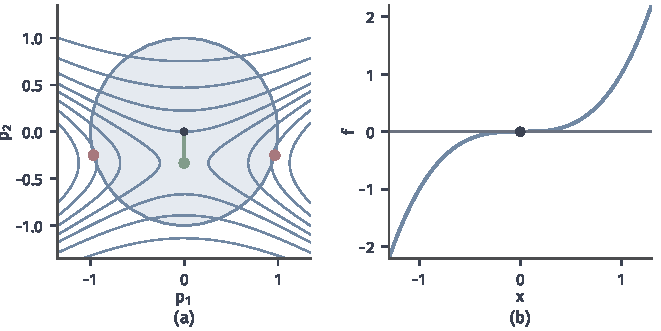
\includegraphics[width=112mm]{figures/05-optimization/02-smooth-optimization/matplotlib/tr-second-order/figure.pdf}
 \caption{二阶保证的两个边界。(a)~模型$\bm{g}=(0,1)^\top$，$\bm{B}=\operatorname{diag}(-1,3)$，$\Delta=1$：截断共轭梯度只沿$p_2$轴走到绿点，两个红点是全局解。(b)~$f(x)=x^3$，黑点处梯度和Hessian都为零，满足二阶必要条件，却不是局部极小点。}
 \label{fig:tr-second-order}
\end{BookInlineFigure}

\paragraph{迭代次数}
定理~\ref{thm:tr-first-order}的证明本身给出了复杂度。设前$T$轮都有$\lVert\bm{g}^{(t)}\rVert_2\geq\varepsilon$，半径有下界$\Delta_{\min}$，$\varepsilon$小时$\Delta_{\min}$与$\varepsilon$同阶。把第四步中每次接受的下降量代入总下降量$f(\bm{x}^{(0)})-f_{\mathrm{low}}$，可知接受的轮数$A$满足
\begin{equation}
 A\leq\frac{f(\bm{x}^{(0)})-f_{\mathrm{low}}}{\eta_1c_1\varepsilon\min\{\Delta_{\min},\ \varepsilon/M\}}=O(\varepsilon^{-2}).
 \label{eq:tr-accepted-count}
\end{equation}

拒绝的轮数$R$也受控制。半径每次接受至多乘以$2$，每次拒绝乘以$\theta$，且始终不低于$\Delta_{\min}$，所以$\Delta^{(0)}2^A\theta^R\geq\Delta_{\min}$，由此得到
\begin{equation}
 R\leq\frac{A\ln2+\ln(\Delta^{(0)}/\Delta_{\min})}{\ln(1/\theta)}.
 \label{eq:tr-rejected-count}
\end{equation}

因此外层总轮数是$O(\varepsilon^{-2})$，只比接受轮数多一个常数倍和一个对数项。这个阶与梯度下降相同，并且对信赖域Newton法也是紧的，构造最坏的目标需要专门设计的例子，篇幅较长，读者可查阅专门的优化复杂度文献。这也提醒我们，信赖域Newton法在实践中的优势来自局部收敛和对曲率的利用，不来自这个最坏情形的上界。

\paragraph{局部收敛}
设$\bm{x}^{(t)}\to\bm{x}^\star$，$\nabla^2f(\bm{x}^\star)\succ\bm{0}$，Hessian在$\bm{x}^\star$附近Lipschitz，并取$\bm{B}^{(t)}=\bm{H}^{(t)}$。靠近解时Newton步趋于零，比值$\rho^{(t)}$趋于$1$，半径不再缩小，Newton步终将落在球内。狗腿法、精确解都直接取Newton步，于是回到第~\ref{chap:second-order-methods}章的局部二次收敛。截断共轭梯度由残差停止，$\eta\to0$的快慢决定超线性或二次收敛，取$\eta=\min\{0.1,\sqrt{\lVert\bm{g}\rVert_2}\}$时是超线性的。表~\ref{tab:tr-history}中第$4$到第$7$轮就是这一阶段。这里只说明了机制，严格的证明还需要验证$\rho^{(t)}\to1$的速度，读者可查阅\scite{math-nocedal2006numerical}。

\paragraph{计算成本}
评价信赖域的成本要把外层和内层分开算，表~\ref{tab:tr-cost}按一次子问题列出。

\begin{BookInlineTable}
 \centering
 \begin{tabular}{lll}
  \toprule
  子问题解法 & 对$\bm{B}$的要求 & 一次求解的代价\\
  \midrule
  Cauchy步 & 对称 & $1$次矩阵向量乘积\\
  狗腿法 & 正定 & $1$次分解，约$n^3/3$\\
  截断共轭梯度 & 对称 & $j$次矩阵向量乘积，$j\leq n$\\
  精确解 & 对称 & 数次分解，约$n^3/3$每次\\
  \bottomrule
 \end{tabular}
 \caption{一次子问题的代价，稠密矩阵，只计主要运算。}
 \label{tab:tr-cost}
\end{BookInlineTable}

外层每一轮需要一次函数值$f(\bm{x}^{(t)}+\bm{p}^{(t)})$；只有被接受的轮才需要新的梯度和$\bm{B}$，拒绝的轮只多一次子问题和一次函数值。Hessian向量乘积不必形成整个矩阵，用梯度差近似时，一次乘积大约是一次梯度的代价：
\begin{equation}
 \bm{H}^{(t)}\bm{v}\approx\frac{\nabla f(\bm{x}^{(t)}+h\bm{v})-\nabla f(\bm{x}^{(t)})}{h}.
 \label{eq:tr-hessian-vector}
\end{equation}
所以比较方法时不能只看外层轮数，要把内层的乘积次数也算进去。拒绝也不是免费的：当函数值很贵时，半径初值和更新因子要避免频繁试探。

图~\ref{fig:tr-methods-compare}是一个$n=20$的实验，目标是
\[
 f(\bm{x})=\sum_{i=1}^{19}\bigl[10(x_{i+1}-x_i^2)^2+(1-x_i)^2\bigr].
\]
三种方法的外层框架相同，参数同前。精确Hessian配截断共轭梯度用$26$个外层轮次、$157$次Hessian向量乘积把梯度降到$10^{-7}$以下。SR1模型从$20\bm{I}$出发，用$90$轮，每轮要多算一次梯度，但完全不用Hessian。只用Cauchy步时，$1200$轮后梯度仍有$1.8\times10^{-4}$。三者都满足第~\ref{sec:tr-convergence}节开头的假设，收敛定理对它们一视同仁，实际差距来自模型和子问题利用了多少曲率。

\begin{BookInlineFigure}
 \centering
 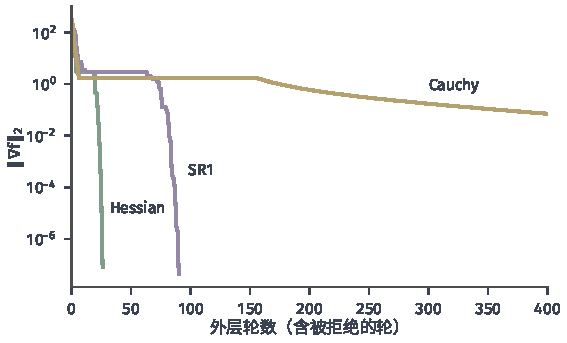
\includegraphics[width=96mm]{figures/05-optimization/02-smooth-optimization/matplotlib/tr-methods-compare/figure.pdf}
 \caption{同一信赖域框架下三种选择的梯度范数（到当前轮为止的最小值，对数坐标）。绿线是Hessian配截断共轭梯度，紫线是SR1模型配截断共轭梯度，黄线是Hessian配Cauchy步。横轴的轮数包含被拒绝的轮。目标是正文中的$20$维函数，每个奇数位分量初值为$-1.2$，其余为$1$。}
 \label{fig:tr-methods-compare}
\end{BookInlineFigure}

\section{本章小结}
\label{sec:tr-summary}

本章开头的问题是：局部模型只在附近可靠，怎样同时决定往哪里走、走多远。信赖域的回答是把两件事合并成一个带半径约束的子问题，半径表示当前愿意相信模型的范围。这样即使曲率矩阵不定，子问题也有解，负曲率不必被修正掉，反而可以把步推向边界。

子问题的全局解由一个平移过的线性方程刻画，但外层迭代并不需要它。Cauchy步给出充分模型下降的下限，狗腿法在$\bm{B}$正定时用两段折线逼近解的轨迹，截断共轭梯度只用矩阵向量乘积，并用边界和曲率两条规则处理信赖域带来的新情况。

下降比$\rho^{(t)}$把模型的预测和目标的实际下降作比较，决定接受这一步以及下一轮的半径。拒绝时点不动，模型沿用，只在更小的范围内重解。

收敛分析的条件和结论要分开记。目标下有界、梯度Lipschitz、模型有界、充分模型下降，这四条保证梯度趋于零，外层轮数是$O(\varepsilon^{-2})$，并不要求精确的Hessian。取精确Hessian并要求候选步利用负曲率，才有二阶必要条件的保证，而这仍不等于找到局部极小点，更不等于全局最优。

表~\ref{tab:tr-summary}把三种子问题解法放在一起。

\begin{BookInlineTable}
 \centering
 \begin{tabular}{llll}
  \toprule
  解法 & $\bm{B}$的要求 & 主要代价 & 负曲率\\
  \midrule
  Cauchy步 & 对称 & 一次乘积 & 只看负梯度方向\\
  狗腿法 & 正定 & 一次分解 & 不能处理\\
  截断共轭梯度 & 对称 & 若干次乘积 & 遇到时走到边界\\
  全局解 & 对称 & 数次分解 & 完整利用\\
  \bottomrule
 \end{tabular}
 \caption{子问题几种解法的对照。}
 \label{tab:tr-summary}
\end{BookInlineTable}

最后一列是第~\ref{chap:saddle-points}章的入口。模型处理负曲率的能力只是工具，梯度很小时所得驻点属于哪一种，怎样可靠地离开鞍点，要在那里进一步明确。

